\section{Experimental Details}
\label{appendix_sec:experimental_details}

\paragraph{Tasks} We evaluate Rainbow on 20 games from the Arcade Learning Environment \citep{bellemare2013arcade}. We use the same set of games evaluated by \citet{ceron2024mixtures} for direct comparison. This includes: Asterix, SpaceInvaders, Breakout, Pong, Qbert, DemonAttack, Seaquest, WizardOfWor, RoadRunner, BeamRider, Frostbite, CrazyClimber, Assault, Krull, Boxing, Jamesbond, Kangaroo, UpNDown, Gopher, and Hero.  In addition, we run some of our main results on all suite of $60$ games. 

On Atari100k benchmark, we evaluate on the full $26$ games. These are: Alien, Amidar, Assault, Asterix, BankHeist, BattleZone, Boxing, Breakout, ChopperCommand, CrazyClimber, DemonAttack, Freeway, Frostbite, Gopher, Hero, Jamesbond, Kangaroo, Krull, KungFuMaster, MsPacman, Pong, PrivateEye, Qbert, RoadRunner, Seaquest, UpNDown.


\paragraph{Hyper-parameters} We use the default hyper-parameter values for DQN \citep{mnih2015humanlevel}, Rainbow \citep{hessel2018rainbow}, and DER \citep{van2019use} agents. We share the details of these values in \autoref{tbl:defaultvalues}.

\begin{table}[!h]
 \centering
  \caption{Default hyper-parameters setting for DQN, Rainbow and DER agents.}
  \label{tbl:defaultvalues}
 \begin{tabular}{@{} cccc @{}}
  %\toprule
    \toprule
    & \multicolumn{3}{c}{Atari}\\
    \cmidrule(lr){2-4}
  Hyper-parameter &  DQN & Rainbow & DER\\
    \midrule
     Adam's ($\epsilon$) & 1.5e-4 & 1.5e-4 & 0.00015\\
     Adam's learning rate &  6.25e-5 & 6.25e-5 & 0.0001\\
     Batch Size & 32 & 32 & 32\\
     Conv. Activation Function & ReLU & ReLU & ReLU\\
     Convolutional Width & 1 & 1 &\\
     Dense Activation Function & ReLU & ReLU & ReLU\\
     Dense Width & 512 & 512 & 512\\
     Normalization & None & None & None\\
     Discount Factor & 0.99 & 0.99 & 0.99 \\
     Exploration $\epsilon$ & 0.01 & 0.01 & 0.01\\
     Exploration $\epsilon$ decay & 250000 & 250000 & 2000\\
     Minimum Replay History & 20000 & 20000& 1600\\
     Number of Atoms & 0 & 51 & 51 \\
     Number of Convolutional Layers & 3 & 3 & 3\\
     Number of Dense Layers & 2 & 2& 2\\
     Replay Capacity & 1000000 & 1000000& 1000000 \\
     Reward Clipping & True & True & True\\
     Update Horizon & 1 & 3 & 10\\
     Update Period & 4 & 4 &  1\\
     Weight Decay & 0 & 0 & 0\\
     Sticky Actions & True & True & False\\
     \bottomrule
  \end{tabular}
\end{table}


\section{Additional Experiments}
\subsection{Comparison between token choice routing and expert choice routing}
\label{appendix_sec:expertChoicevsTokenChoice}

We focus in our analysis on expert choice routing, where experts select tokens, as opposed to token choice routing, where tokens select experts. We compare these two routing strategies across different numbers of experts using a Rainbow agent with a ResNet architecture.

\autoref{fig:tokenvsexpert} demonstrates that expert choice routing consistently outperforms token choice routing across varying number of experts.  Moreover, this performance gap widens as the number of experts increases, highlighting the advantages of expert choice routing in addressing the limitations of token choice routing.

\begin{figure}[h!]
    \centering
    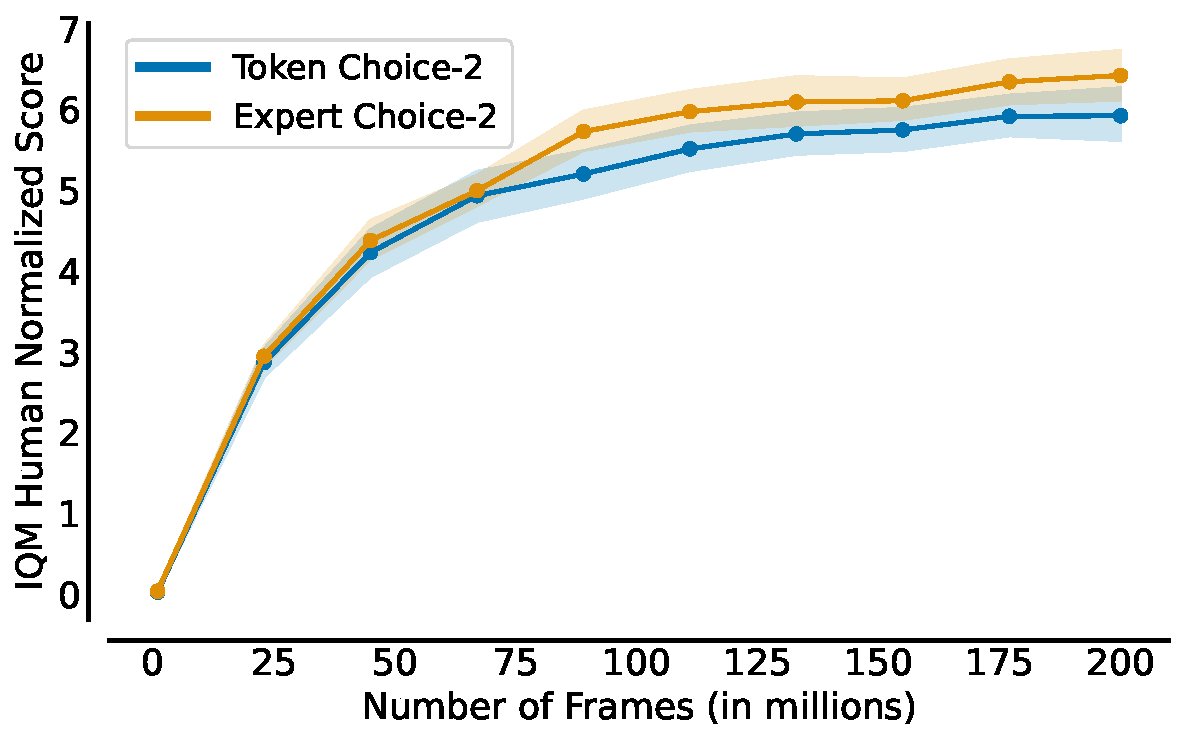
\includegraphics[width=0.4\textwidth]{figures/results/TokenChoiceVsExpertChoice-2.pdf}
    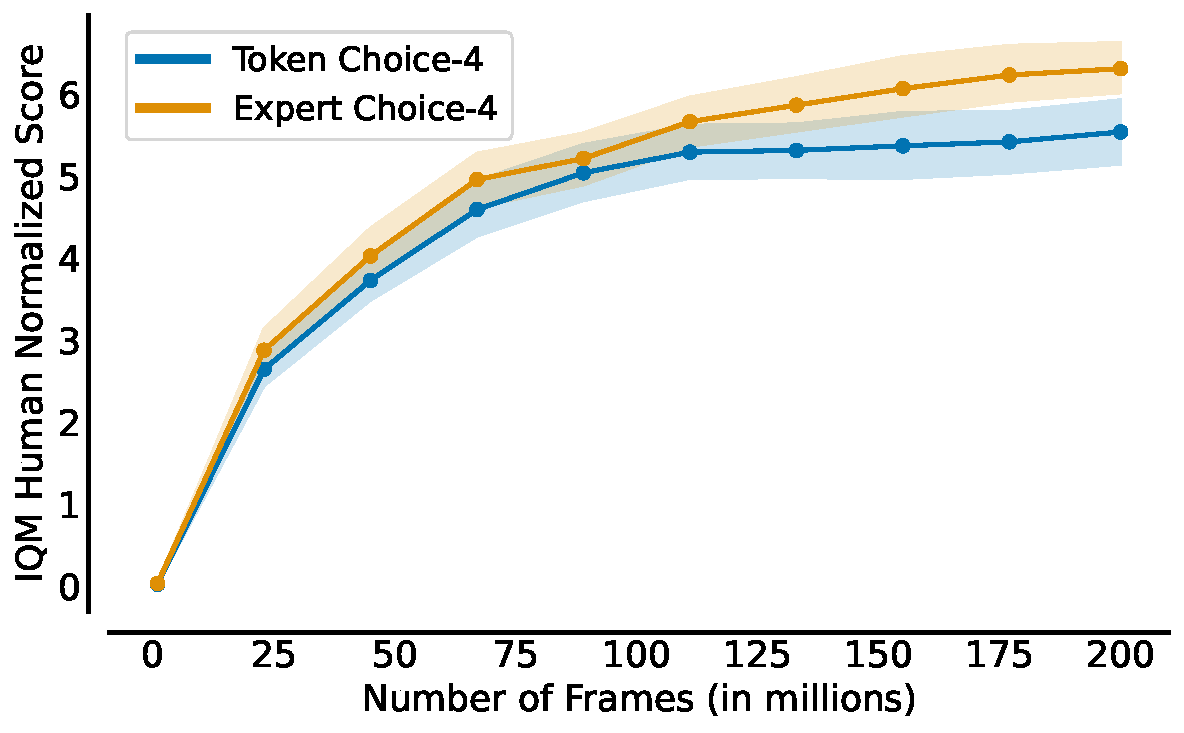
\includegraphics[width=0.4\textwidth]{figures/results/TokenChoiceVsExpertChoice-4.pdf}
    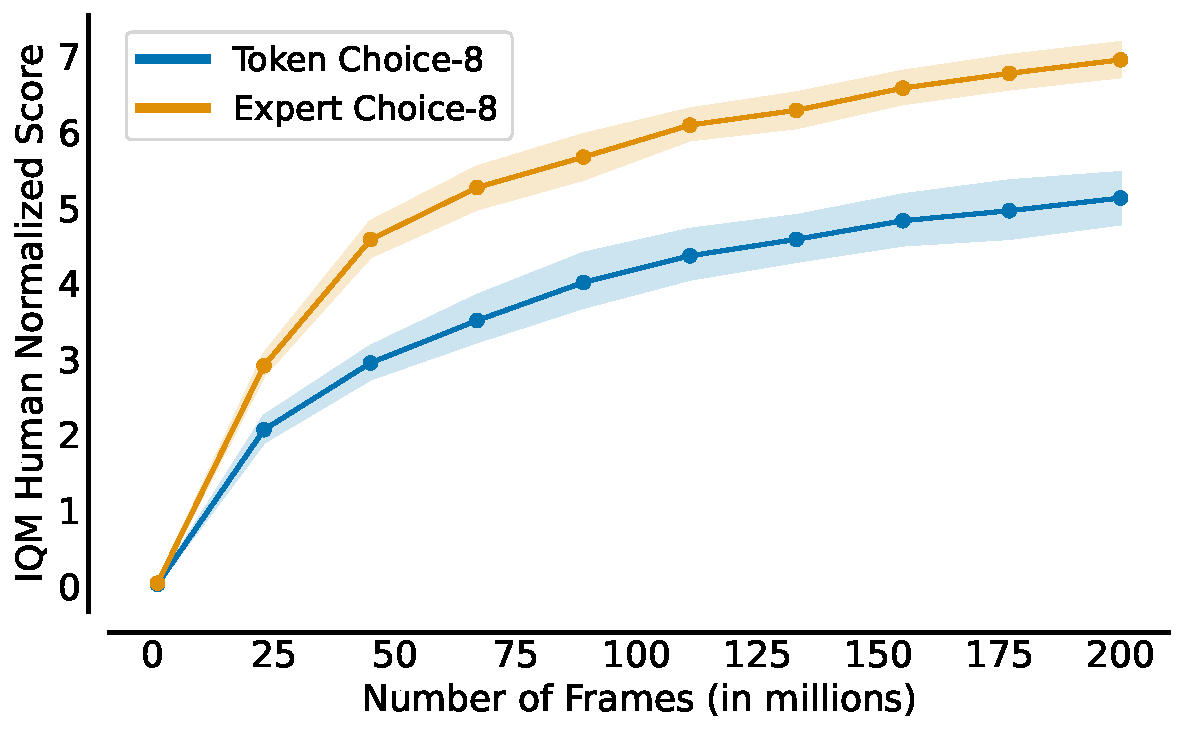
\includegraphics[width=0.4\textwidth]{figures/results/TokenChoiceVsExpertChoice-8.pdf}
    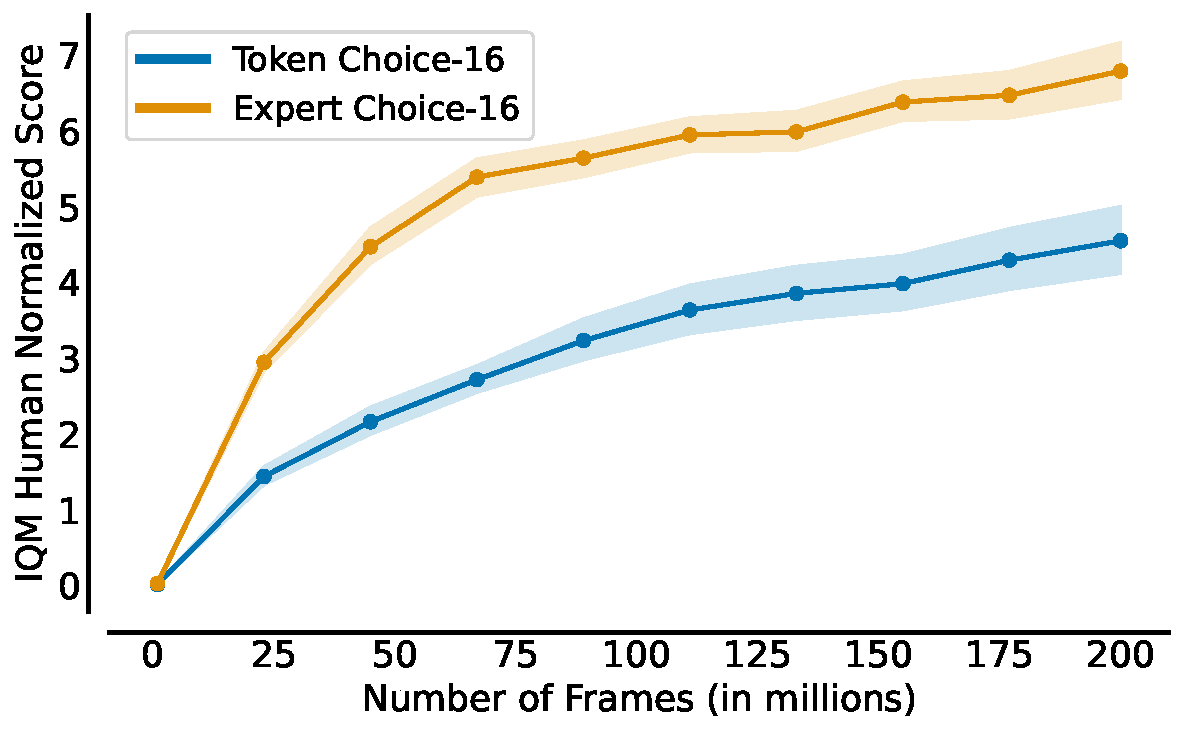
\includegraphics[width=0.4\textwidth]{figures/results/TokenChoiceVsExpertChoice-16.pdf}
    \vspace{-0.4cm}
    \caption{A comparison between token choice routing and expert choice routing on Rainbow with ResNet encoder. Expert choice routing consistently outperforms token choice routing across different number of experts. We report interquantile mean performance with error bars indicating 95\% confidence intervals, over 20 games with 5 seeds each.}
    \label{fig:tokenvsexpert}
    \vspace{-0.2cm}
\end{figure}

\newpage

\subsection{Don't flatten tokenize}
\label{appendix:don'tFlatten}
In this section, we provide further analysis on the impact of tokenization and their weight combination on models with \rebuttal{varying number of experts}. To this end, we investigate \rebuttal{SoftMoE-2} and SoftMoE-8 and compare it against the scaled SoftMoE-1 and ExpertChoice-1 (non-combined tokenization). \autoref{fig:tokenImapct_8experts} shows that single scaled expert can reach a performance close to multiple experts, even in the case of large number of experts. In addition, consistent with our results, combined tokenization adds benefits over the sparse one. \autoref{fig:learningcurves_1expert} shows a comparison between the learning curves of single scaled expert and multiple ones.

\begin{figure}[h!]
    \centering
    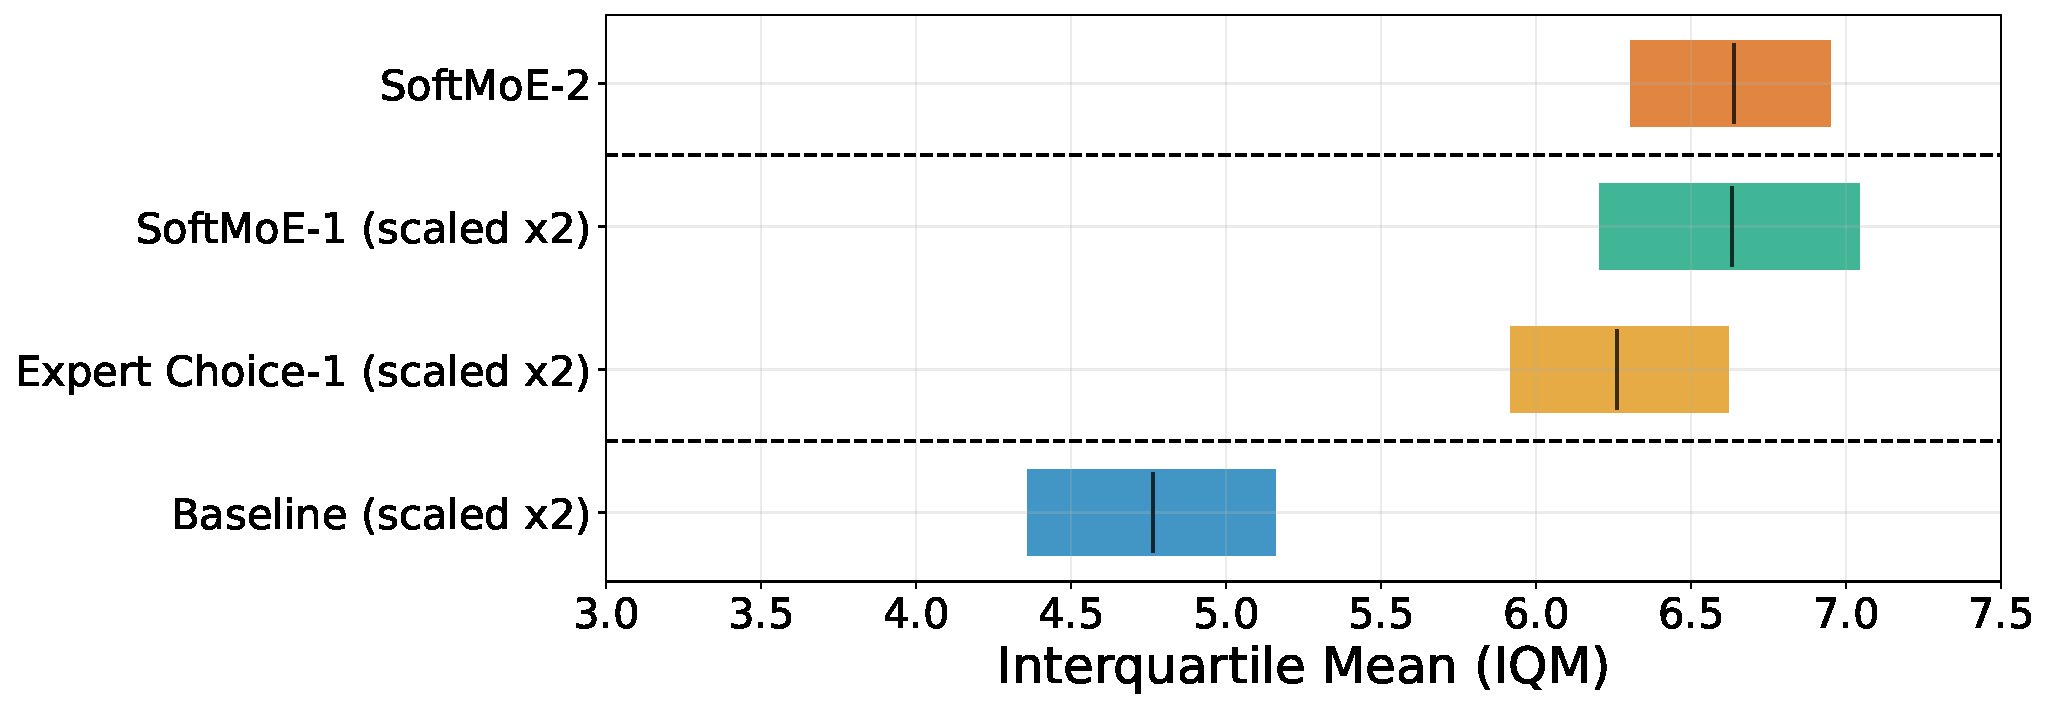
\includegraphics[width=0.7\textwidth]{figures/results/section5_aggregate_v2_2experts.pdf}
    \vspace{-0.4cm}
    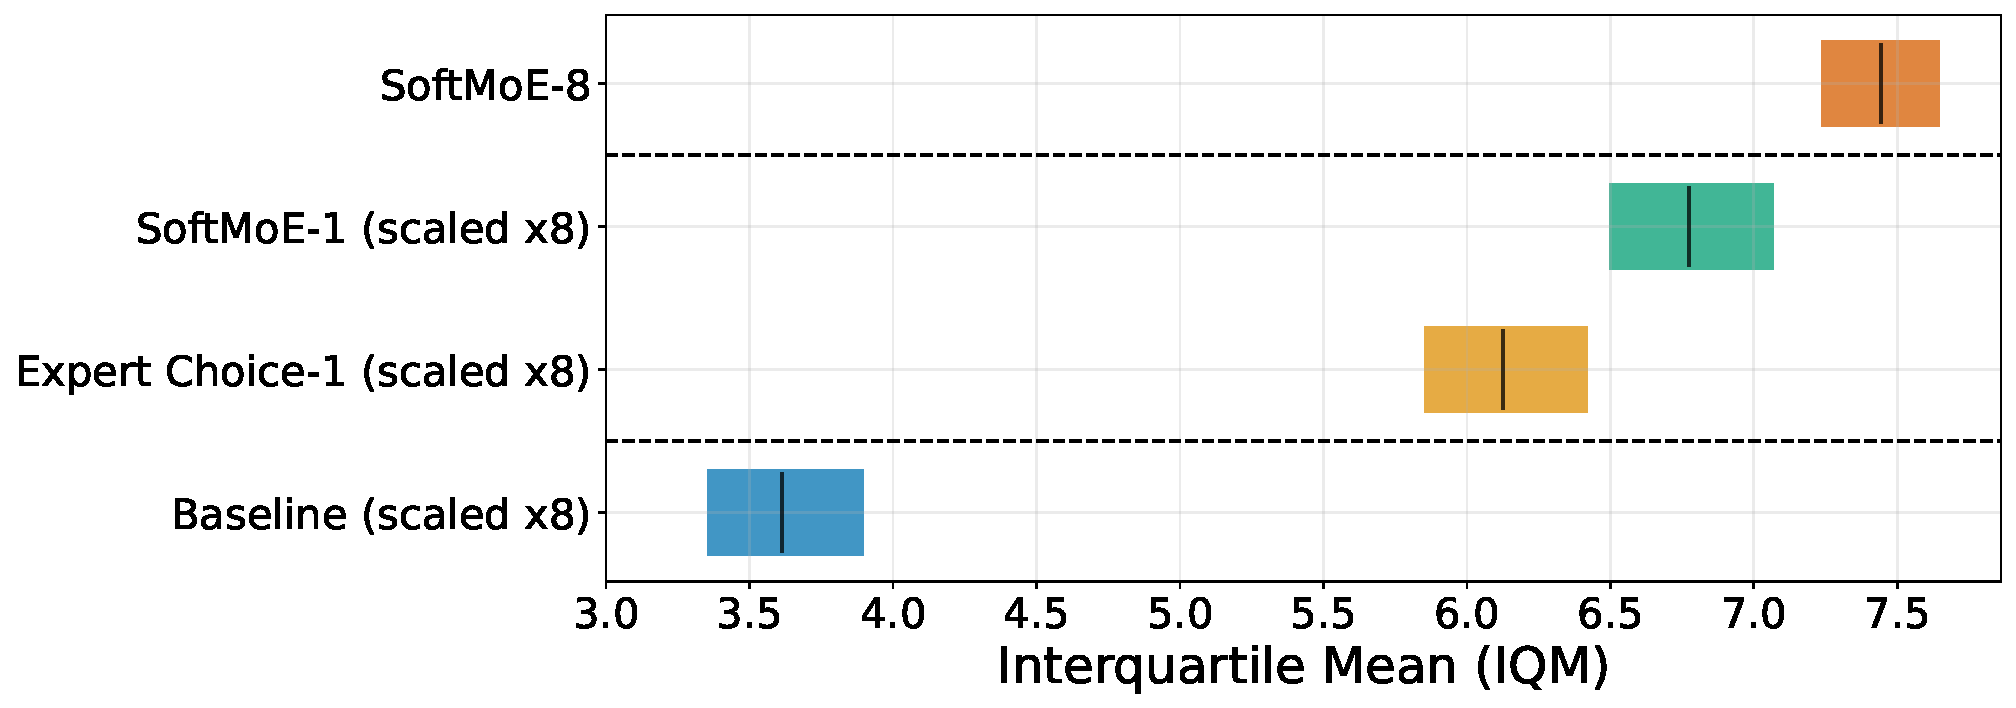
\includegraphics[width=0.7\textwidth]{figures/results/section5_aggregate_v2_8experts.pdf}
    %\vspace{-0.4cm}
    \caption{\rebuttal{Combined tokenization plays a crucial role in performance. SoftMoE-1 with scaled hidden layer achieves a comparable performance to the standard SoftMoE.}}
    \label{fig:tokenImapct_8experts}
    \vspace{-0.2cm}
\end{figure}

\begin{figure}[h!]
    \centering
    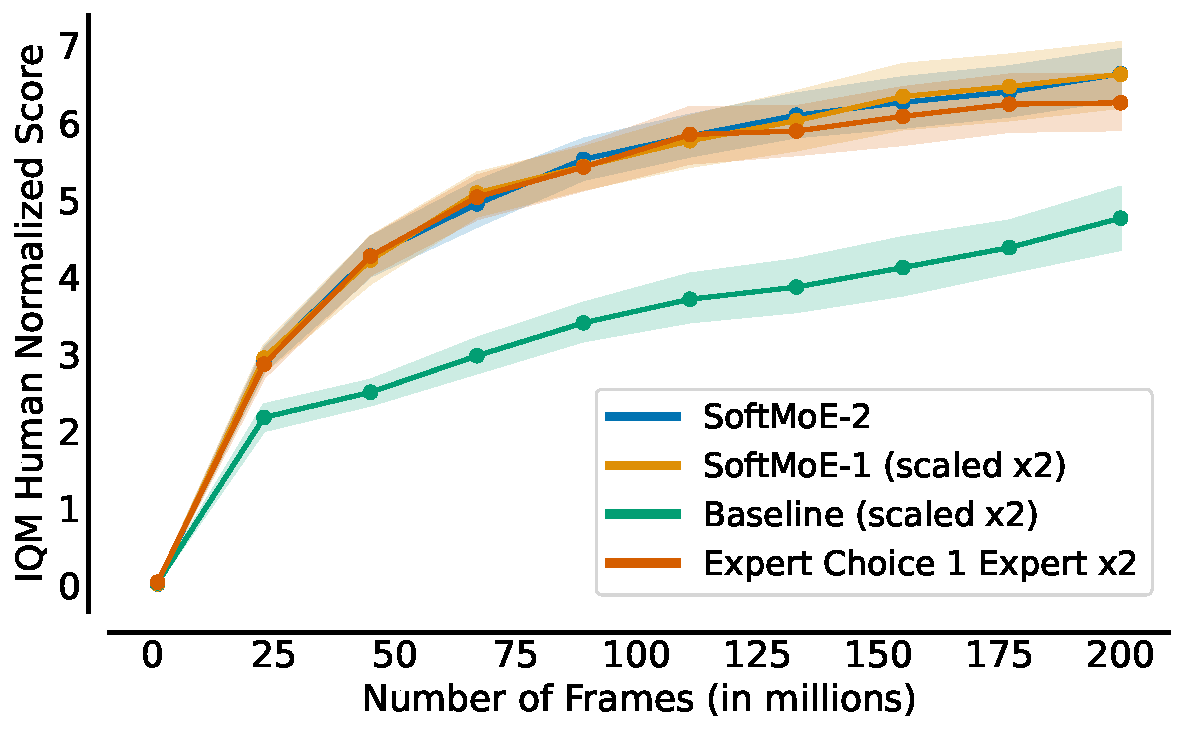
\includegraphics[width=0.3\textwidth]{figures/results/SoftMoE-1_x2.pdf}
    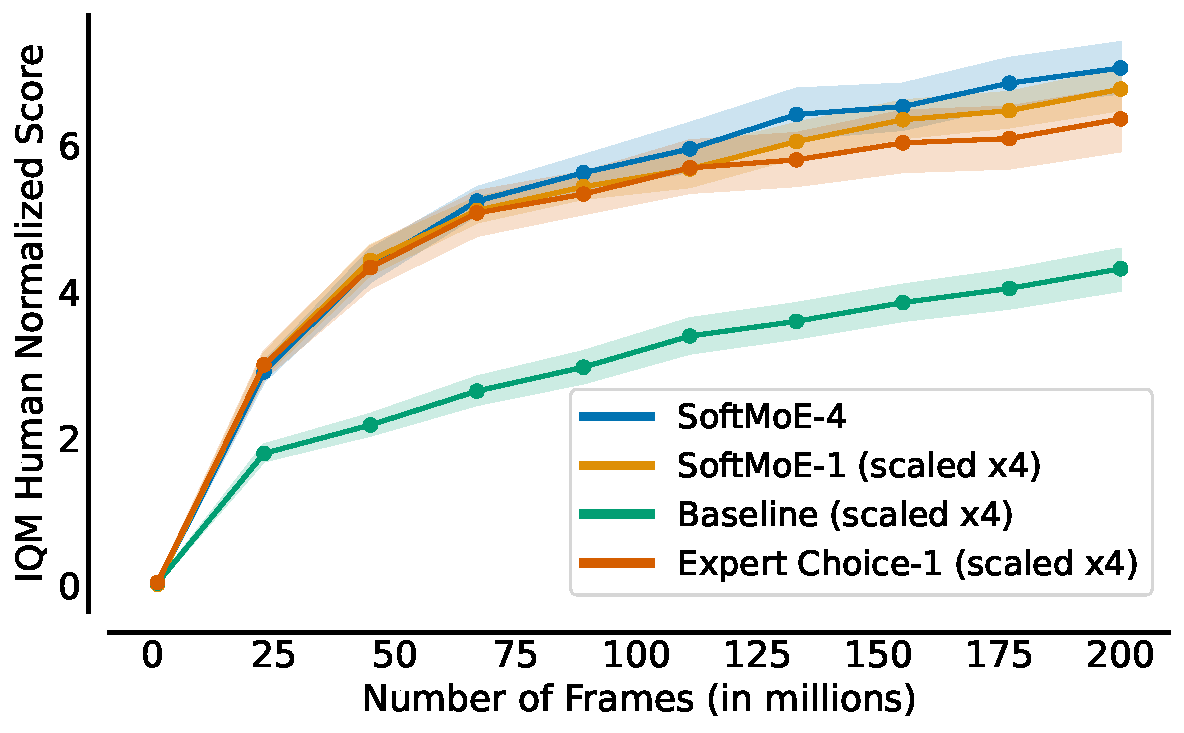
\includegraphics[width=0.3\textwidth]{figures/results/SoftMoE-1_x4.pdf}
        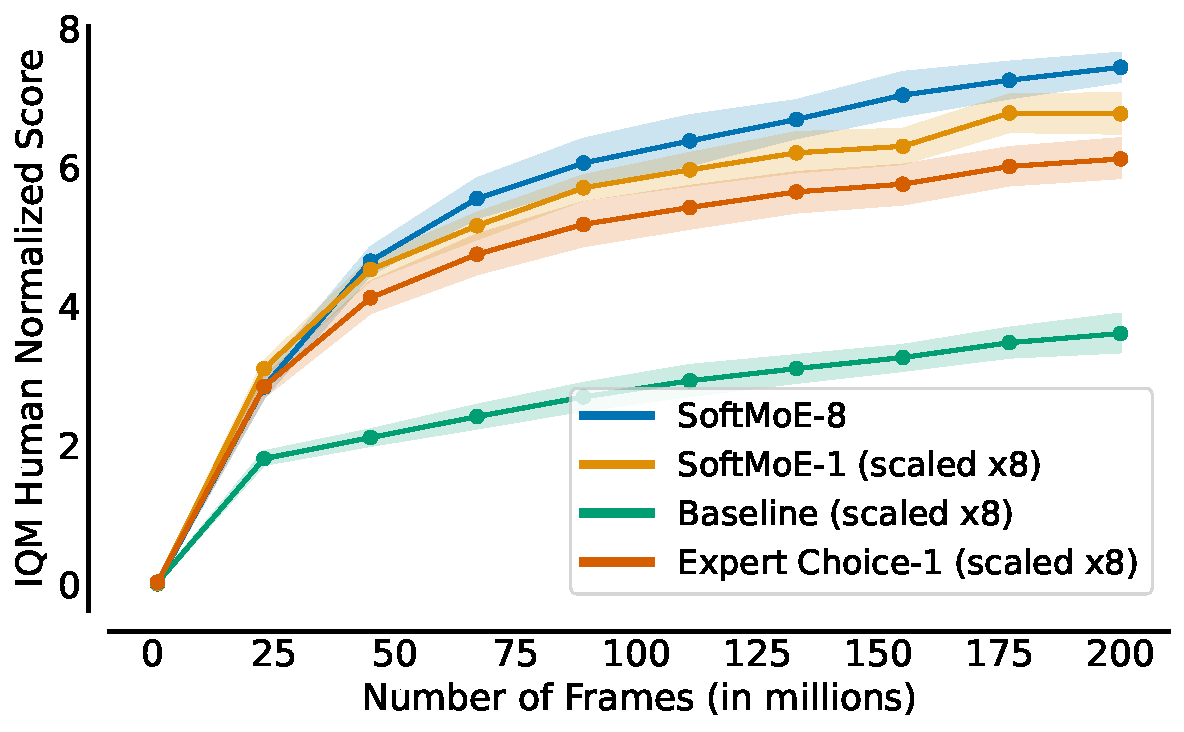
\includegraphics[width=0.3\textwidth]{figures/results/SoftMoE-1_x8.pdf}
    %\vspace{-0.4cm}
    \caption{\rebuttal{Comparison between the learning curves of the scaled SoftMoE-1 and multiple experts. We report interquantile mean performance with error bars indicating 95\% confidence intervals, over 20 games with 5 seeds each.}}
    \label{fig:learningcurves_1expert}
    %\vspace{-0.2cm}
\end{figure}
\newpage

\rebuttal{To further assess the effect of flattening in reducing performance of agents, we replace the flattening operation in the baseline by global average pooling. We performed these experiments on the baseline with the default dimensionality and the scaled one in Rainbow.}

\begin{figure}[h!]
    \centering
    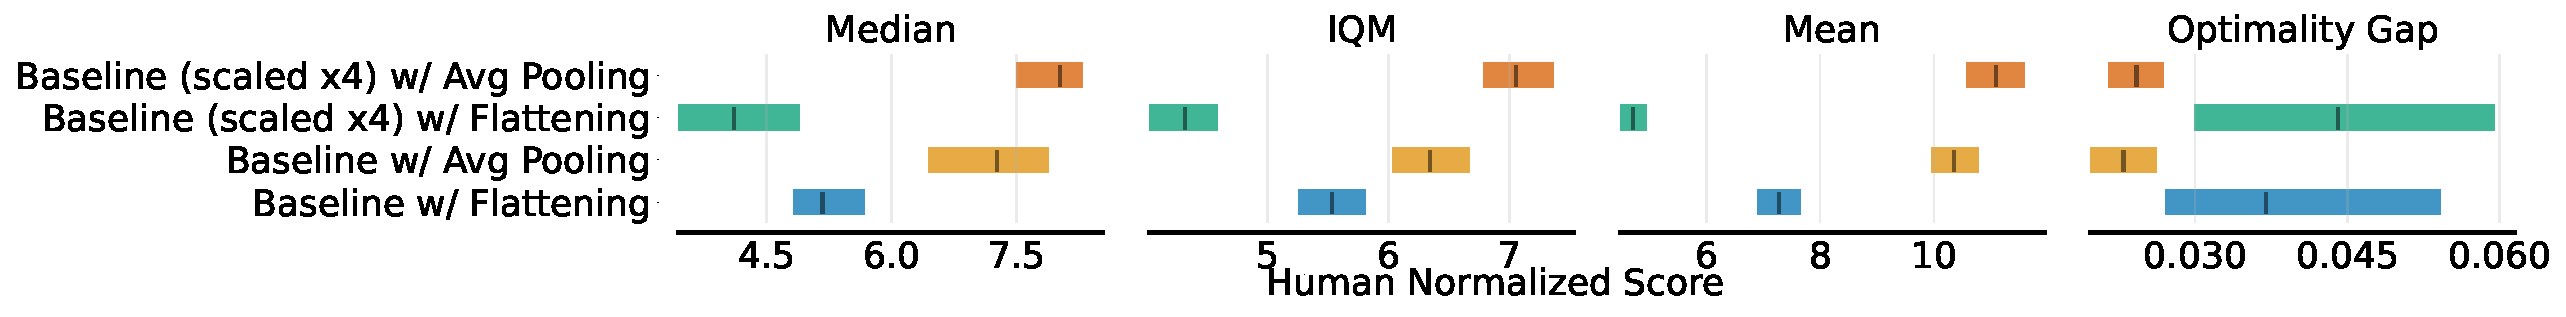
\includegraphics[width=0.9\textwidth]{figures/results/Baselines_avgPool_IntEstimates.pdf}
    %\vspace{-0.4cm}
    \caption{\rebuttal{Replacing the flattening operation by global average pooling improves the performance of the baseline and enables scaling.}}
    \label{fig:baseline_avgpool}
    %\vspace{-0.2cm}
\end{figure}

% \rebuttal{The following figures provide a direct comparison between the unscaled and scaled baselines with their tokenized counterparts.}

% \begin{figure}[!h]
%     \centering
%     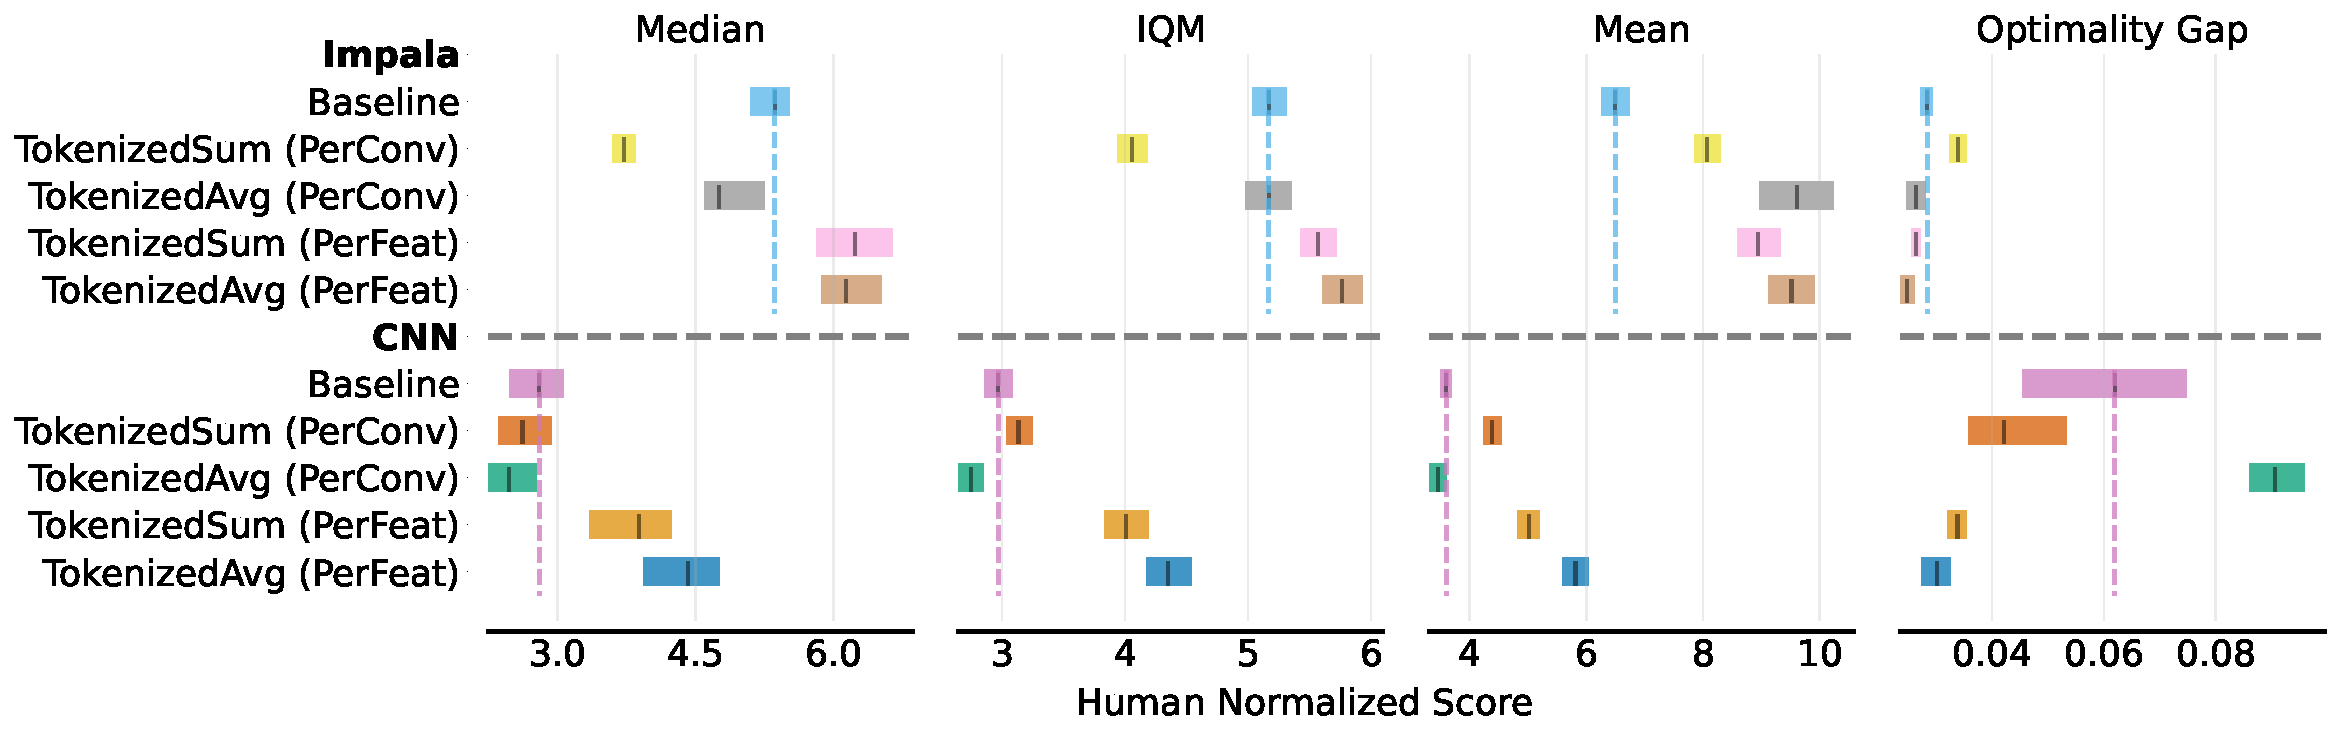
\includegraphics[width=0.8\textwidth]{figures/results/TokenizedRainbowUnscaledRebuttal_IntEstimates.pdf}
%     %\vspace{-0.4cm}
%     \caption{\rebuttal{\textbf{Evaluating impact of tokenizing Rainbow-lite} with Impala (top) and CNN (bottom) architectures, using sum/mean over convolutional features, with no scaling. Reporting Median, IQM, Mean, and Optimaly Gap scores \citep{agarwal2021deep}. Higher is better for all except Optimality Gap.}
%     }
%     \label{fig:unscaledNonMoeTokenized}
%     %\vspace{-0.2cm}
% \end{figure}


% \begin{figure}[!h]
%     \centering
%     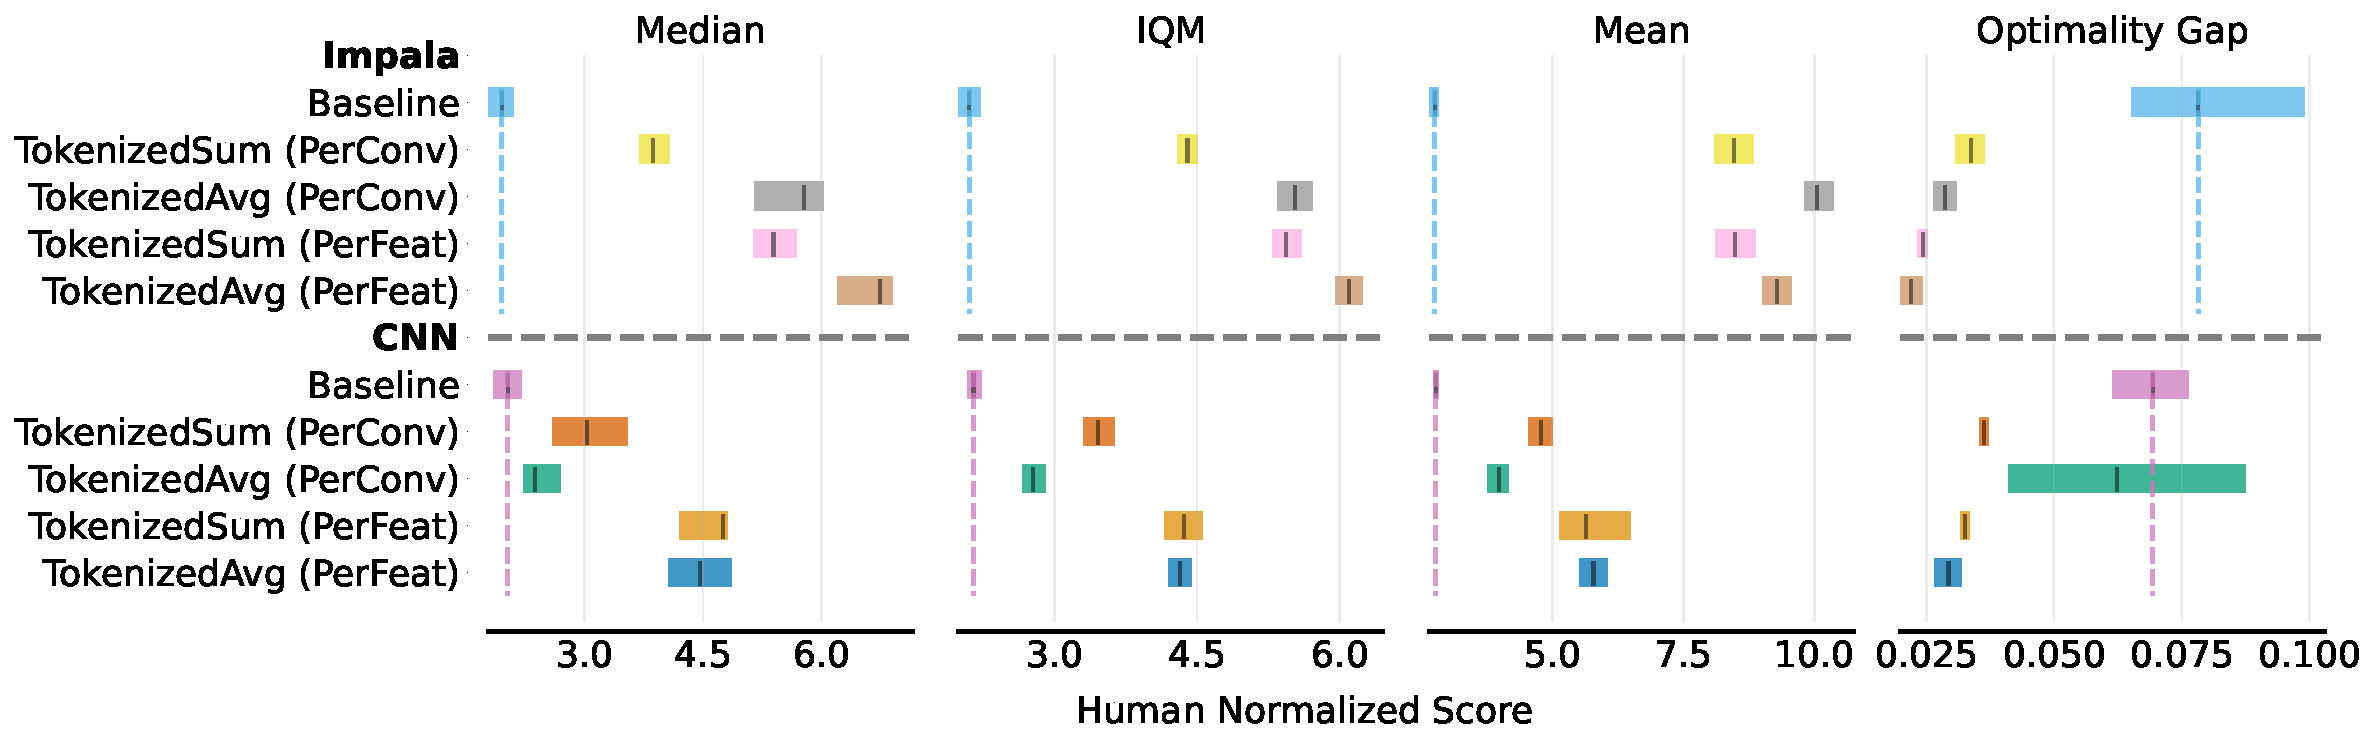
\includegraphics[width=0.8\textwidth]{figures/results/TokenizedRainbowScaledRebuttal_IntEstimates.pdf}
%     %\vspace{-0.4cm}
%     \caption{\rebuttal{\textbf{Evaluating impact of tokenizing Rainbow-lite} with Impala (top) and CNN (bottom) architectures, using sum/mean over convolutional features, with 4x scaling. Reporting Median, IQM, Mean, and Optimaly Gap scores \citep{agarwal2021deep}. Higher is better for all except Optimality Gap.}
%     }
%     \label{fig:scaledNonMoeTokenized}
%     %\vspace{-0.2cm}
% \end{figure}


\subsection{\rebuttal{Analysis of SoftMoE components}}
\label{appendix:analysis_softMoE_components}
\rebuttal{In this section, we present an analysis of each of SoftMoE components on the DER algorithm. As shown in Figure \ref{fig:analysis_softmoe_DER}, we observe similar tends to our findings in Section \ref{sec:anaysis_softmoe_components} on Rainbow. Combined tokens offers an additional benefits over the sparse ones. Experts do seem not be specialized in subset of the tokens. Adjusting the architectural depth and width for direct comparison with the baseline doesn't explain the performance gains of SoftMoE.}

\begin{figure}[h!]
    \centering
    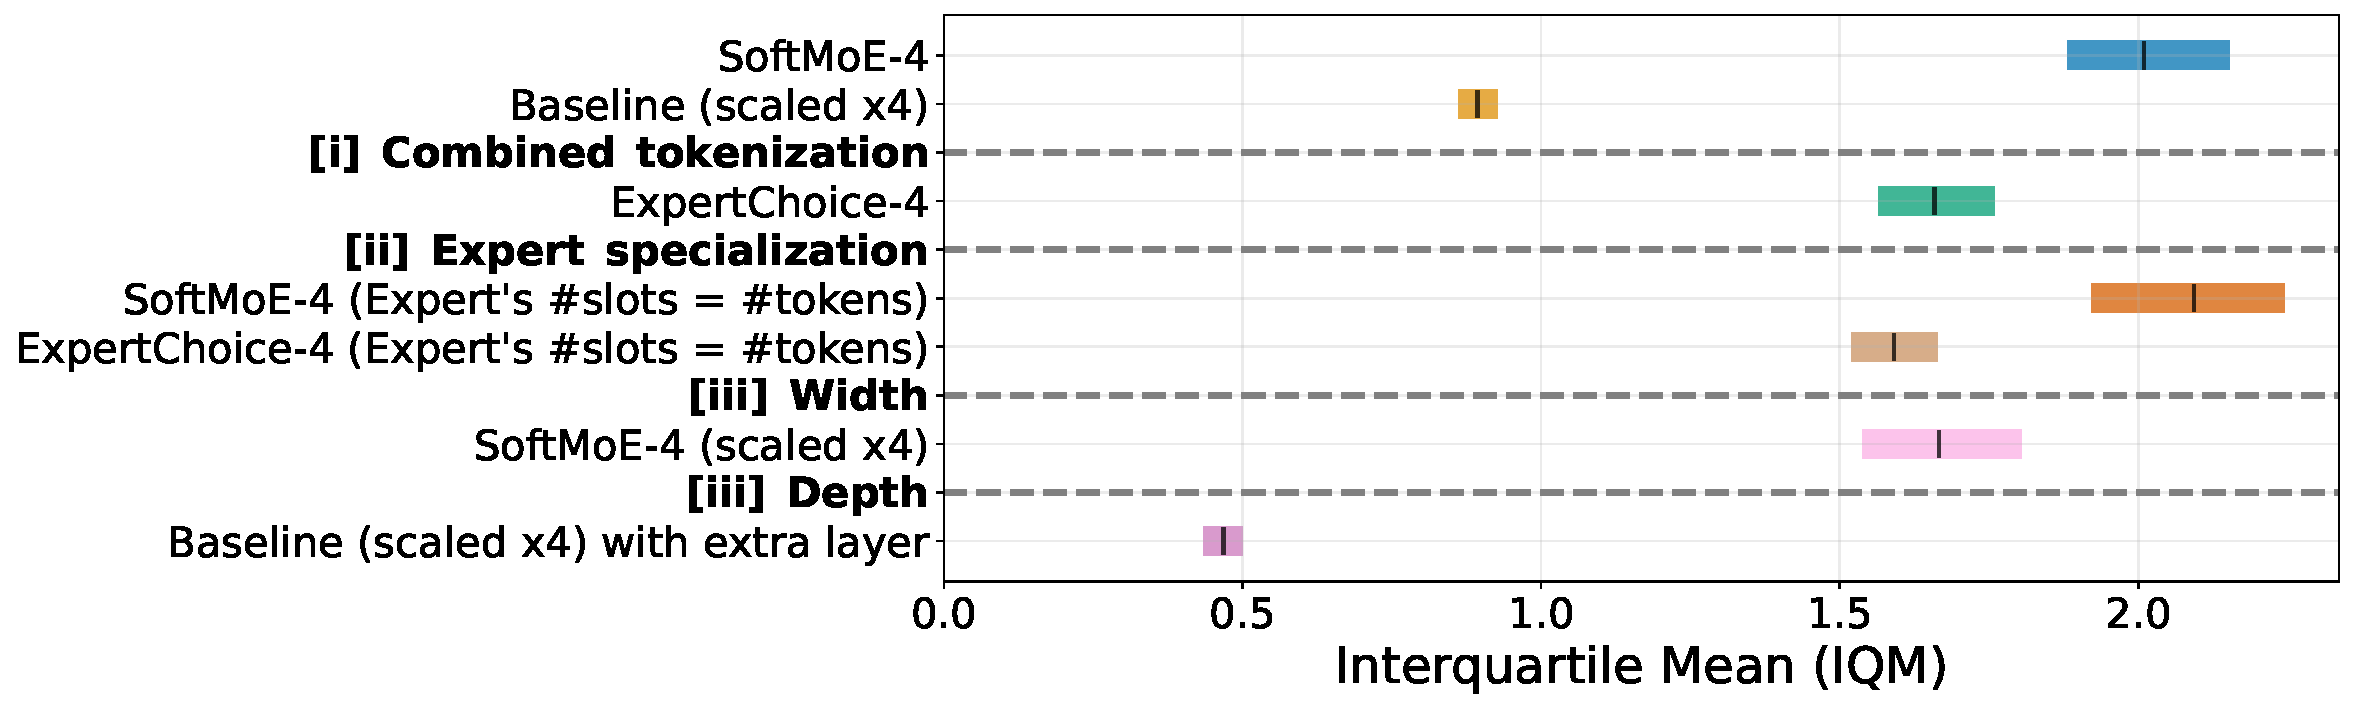
\includegraphics[width=0.8\textwidth]{figures/results/section4_DER_aggregate_v2.pdf}

    \vspace{-0.4cm}
    \caption{\rebuttal{Understanding the impact of SoftMoE components on DER.}}
    \label{fig:analysis_softmoe_DER}
    \vspace{-0.2cm}
\end{figure}

\paragraph{\rebuttal{Effect of Expert width}}
\rebuttal{In section \ref{sec:don'tflatten}, we studied the effect of scaling up the size of the expert hidden layer of SoftMoE-1. Here, we present the results of scaling down the size of this layer by 4. As shown in Figure \ref{fig:analysis_scaledown_SoftMoE-1}, SoftMoE-1 with scaled down layer still outperform the baseline despite that it has less parameter count. }

\begin{figure}[h!]
    \centering
    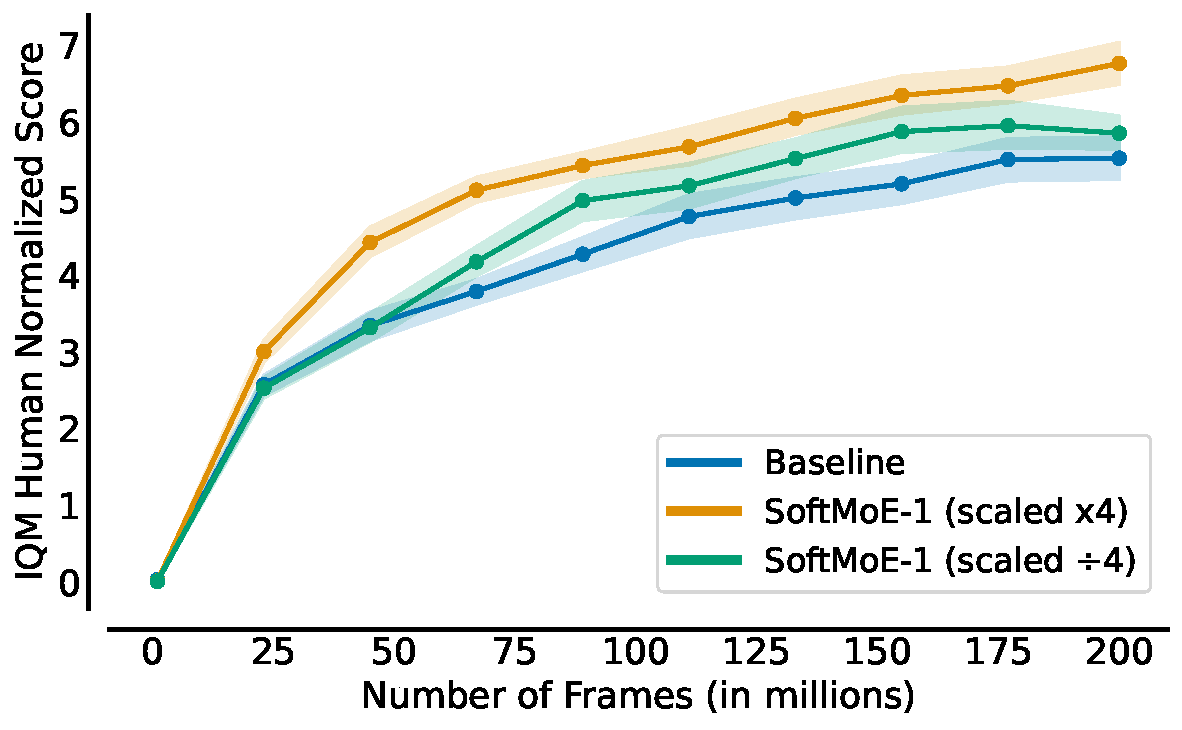
\includegraphics[width=0.4\textwidth]{figures/results/Baselines_scaled_down.pdf}

    \vspace{-0.4cm}
    \caption{\rebuttal{The effect of scaling down the size of the expert hidden layer in SoftMoE-1.}}
    \label{fig:analysis_scaledown_SoftMoE-1}
    \vspace{-0.2cm}
\end{figure}


\subsection{More agents}
Same as our finding for DQN using SoftMoE-4, we observe that single expert has a closer performance to the scaled baseline than SoftMoE-8, as shown in \autoref{fig:DQN_8}. Further investigation is needed to fully understand the behavior of SoftMoE on DQN.


\begin{figure}[!h]
    \centering
    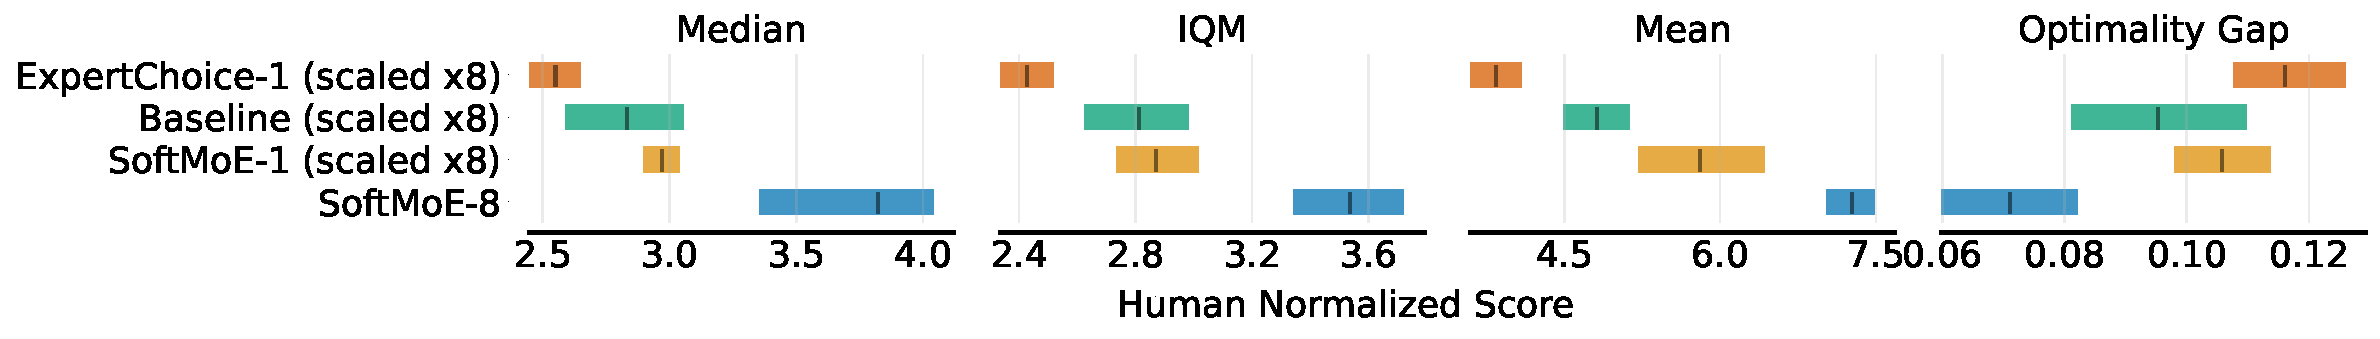
\includegraphics[width=0.95\textwidth]{figures/results/SoftMoE-8_DQN_IntEstimates.pdf}
    %\includegraphics[width=0.95\textwidth]{figures/results/SoftMoE-8_DER_IntEstimates.pdf}
    %\vspace{-0.4cm}
    \caption{Evaluating more agents. When combined with DQN, SoftMoE with a single scaled expert does not provide large gains over the baseline. %In contrast, when combined with DER, it achieves performance comparable to SoftMoE-8 (bottom).
    }
    \label{fig:DQN_8}
    \vspace{-0.2cm}
\end{figure}

\subsection{Expert Utilization}
\label{appendix_sec:expertUtilization}
In this section we provide more analysis to understand the utilization of experts in multi expert setting and the effect of existing techniques on improving plasticity. 

\subsubsection{Some experts are redundant} In Section \ref{sec:anaysis_softmoe_components}, we showed that experts are not specialized in learning subset of tokens. We expand this analysis by assessing the redundancy of experts. To this end, we prune two experts of SoftMoE-4 during training. We studied two pruning schemes: pruning the two experts once and gradually prune throughout training. As shown in \autoref{fig:pruning}, pruning these experts does not change the performance of the agent.


\begin{figure}[!h]
    \centering
    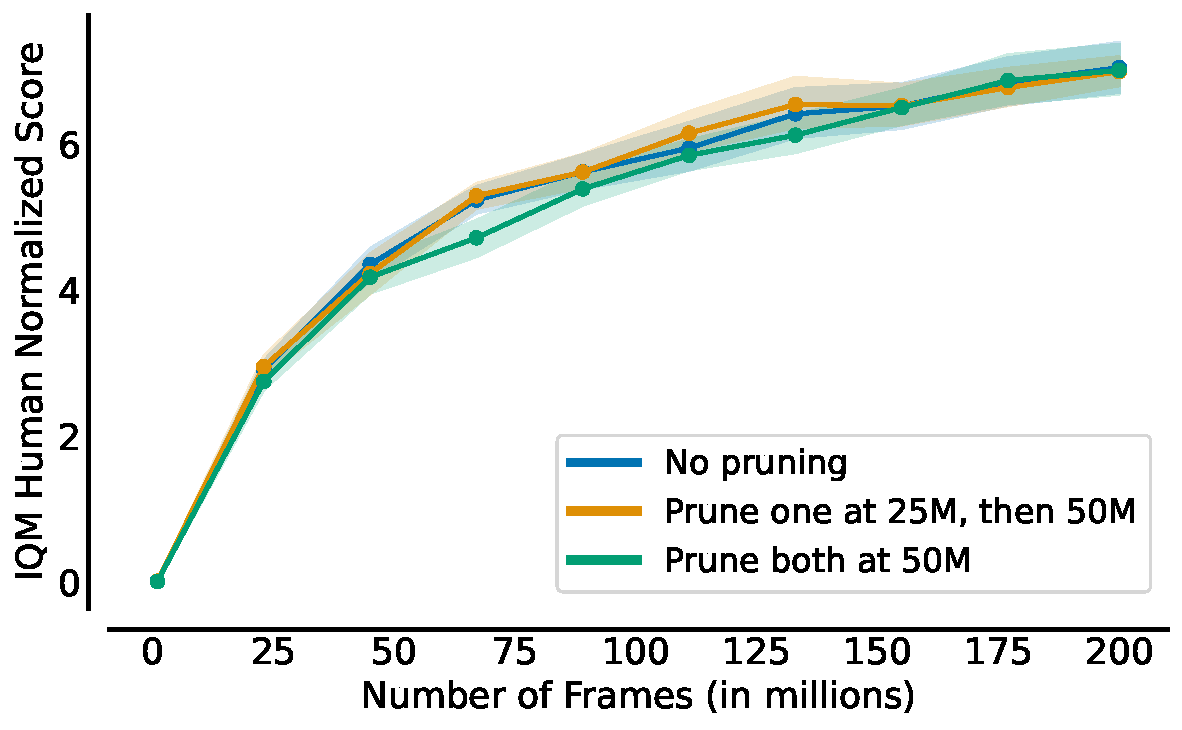
\includegraphics[width=0.5\textwidth]{figures/results/SoftMoE-4-ExpertsPruning.pdf}
    \vspace{-0.4cm}
    \caption{Pruning subset of experts in SoftMoE-4 does not lead to performance drop, suggesting that some of the experts are redundant. We report interquantile mean performance with error bars indicating 95\% confidence intervals, over 20 games with 5 seeds each.}
    \label{fig:pruning}
    %\vspace{-0.2cm}
\end{figure}

\subsubsection{Improving Expert Utilization}
\rebuttal{\paragraph{Experimental details} For
hyper-parameter tuning, we used six games (Asterix, Demon Attack, Seaquest, Breakout, Beam Rider, Space Invaders). For the reset period, we searched for Rainbow over the grid [$0.5\times 10^4$, $10\times10^4, 50\times10^4, 100\times10^4, 125\times10^4, 500\times10^4, 1000\times10^4$] gradient steps. The best found is $125\times10^4$, which corresponds to 20M environment steps. For S\&P, we searched over the values [(0.5, 0.5), (0.4, 0.1), (0.8, 0.2)] for shrink and perturb hyperparameters respectively, as studied in \citep{schwarzer23bbf}. We used values of (0.5, 0.5).} 

\paragraph{Reset experts and router weights} In investigating current techniques to improve expert utilization, we explore reset either experts weights only or both experts and router weights. As illustrated in \autoref{fig:reset_expertsvsexpertsandrouter}, both methods do not help in improving utilization in Rainbow and DQN, with resetting the router weights leads to worse performance.

\begin{figure}[h!]
    \centering
    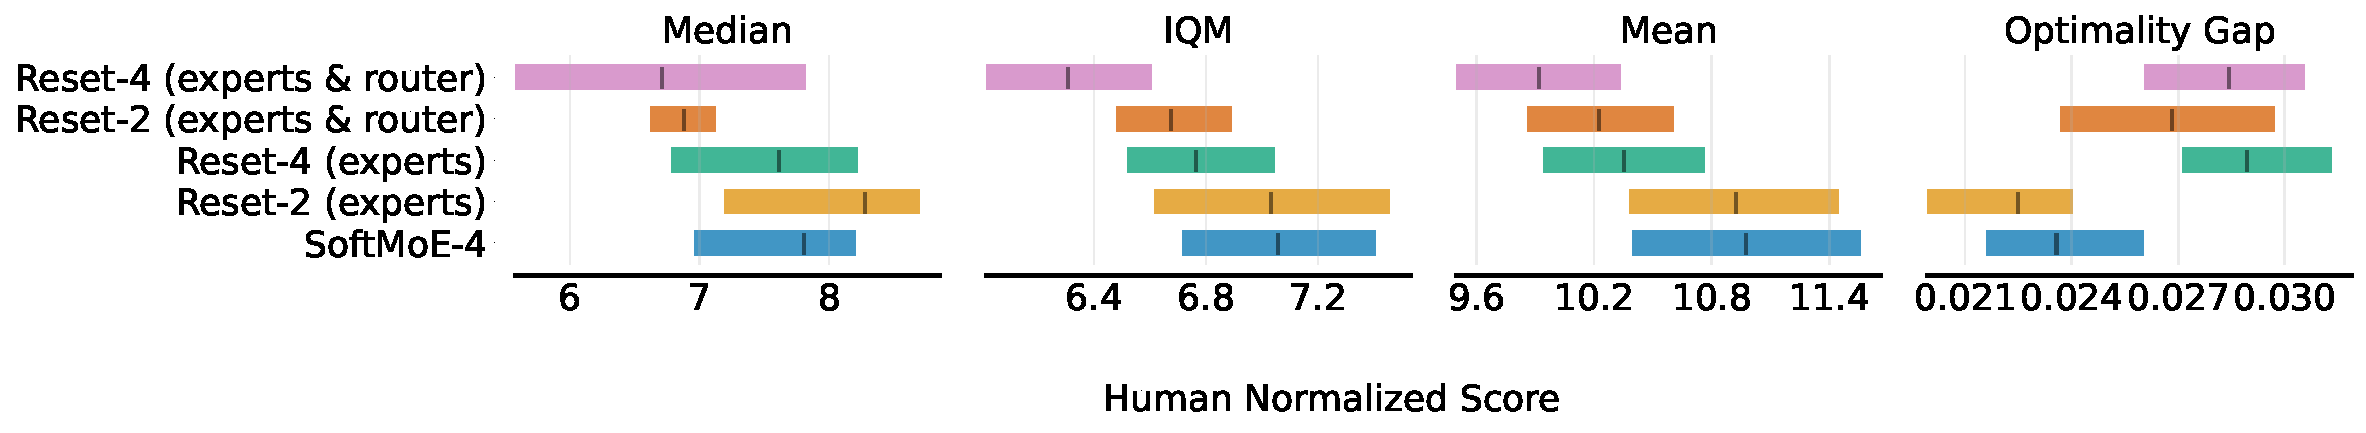
\includegraphics[width=\textwidth]{figures/results/SoftMoE-4_Rainbow-Reset-expertsVSexpertsandrouter_IntEstimates.pdf}
            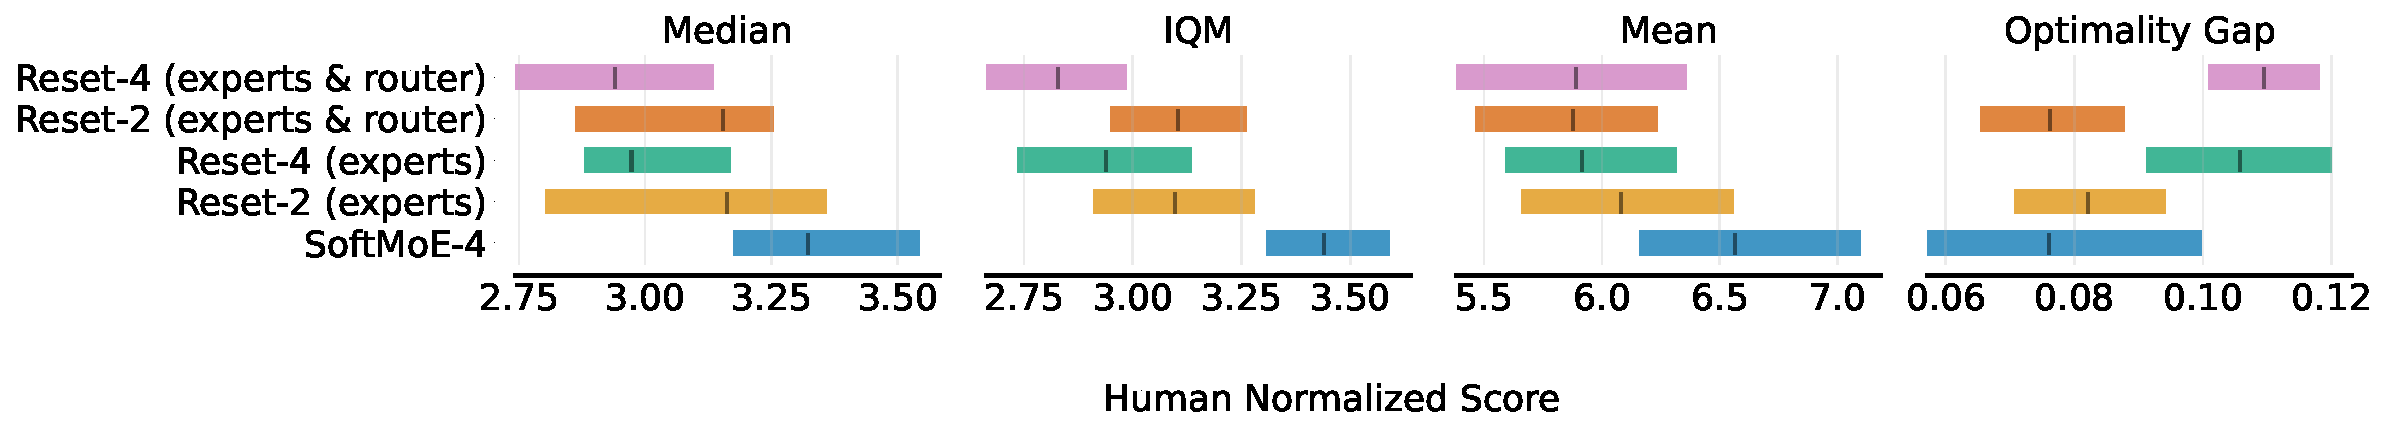
\includegraphics[width=\textwidth]{figures/results/SoftMoE-4_DQN_Reset_weights_only_vs_weightandrouter_IntEstimates.pdf}
        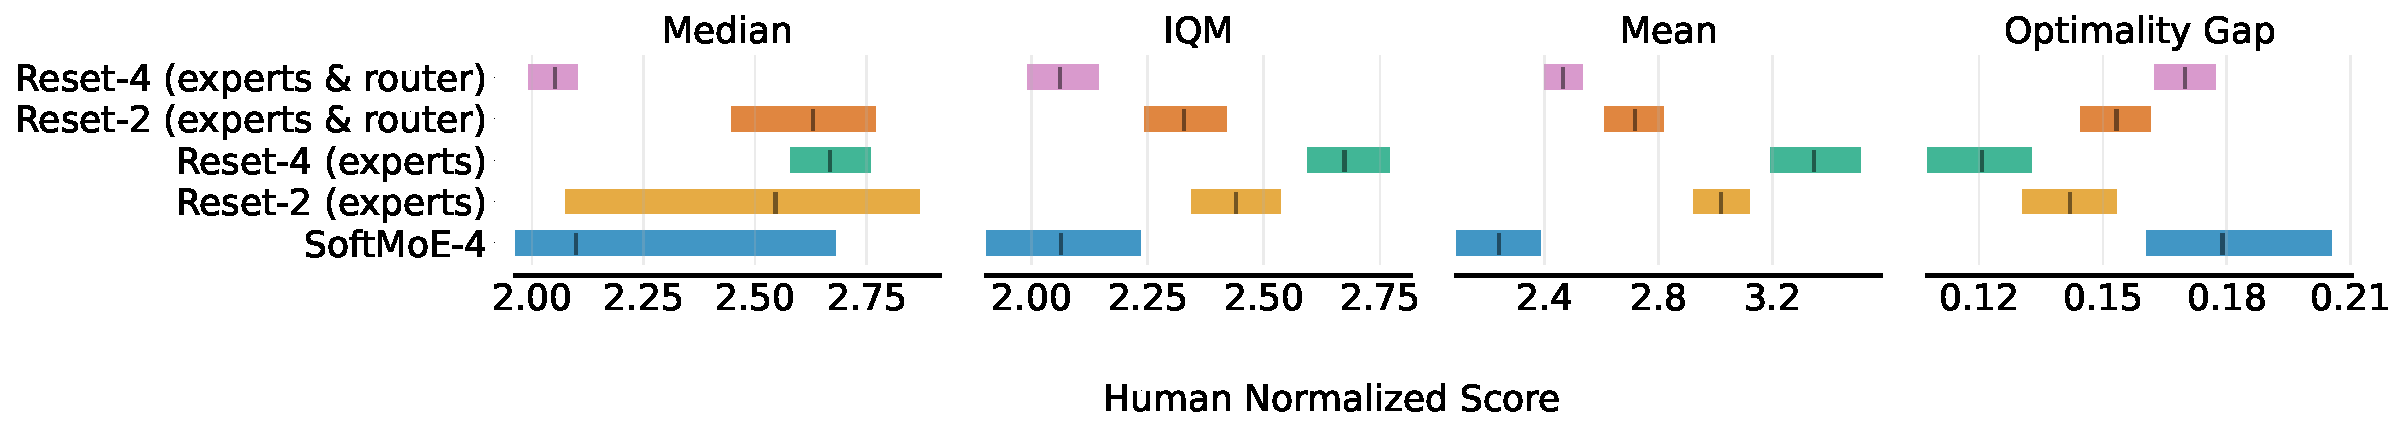
\includegraphics[width=\textwidth]{figures/results/SoftMoE-4_DER-Reset-expertsVSexpertsandrouter_IntEstimates.pdf}
    %\vspace{-0.4cm}
    \caption{Comparison between resetting experts weights only versus experts and router weights in Rainbow (top), \rebuttal{DQN (middle)}, and DER (bottom). }
    \label{fig:reset_expertsvsexpertsandrouter}
    %\vspace{-0.2cm}
\end{figure}

\newpage
\section{\rebuttal{Extra environments}}
\label{sec:appendixExtraEnvs}

\rebuttal{To evaluate the generality of our claims, we conducted experiments with Rainbow on Procgen \citep{cobbe2019procgen} (Figure~\ref{fig:procgenIntEstimates}) and with SAC \citep{haarnoja2018soft} on CALE \citep{farebrother2024cale}.}

\begin{figure}[h!]
    \centering
    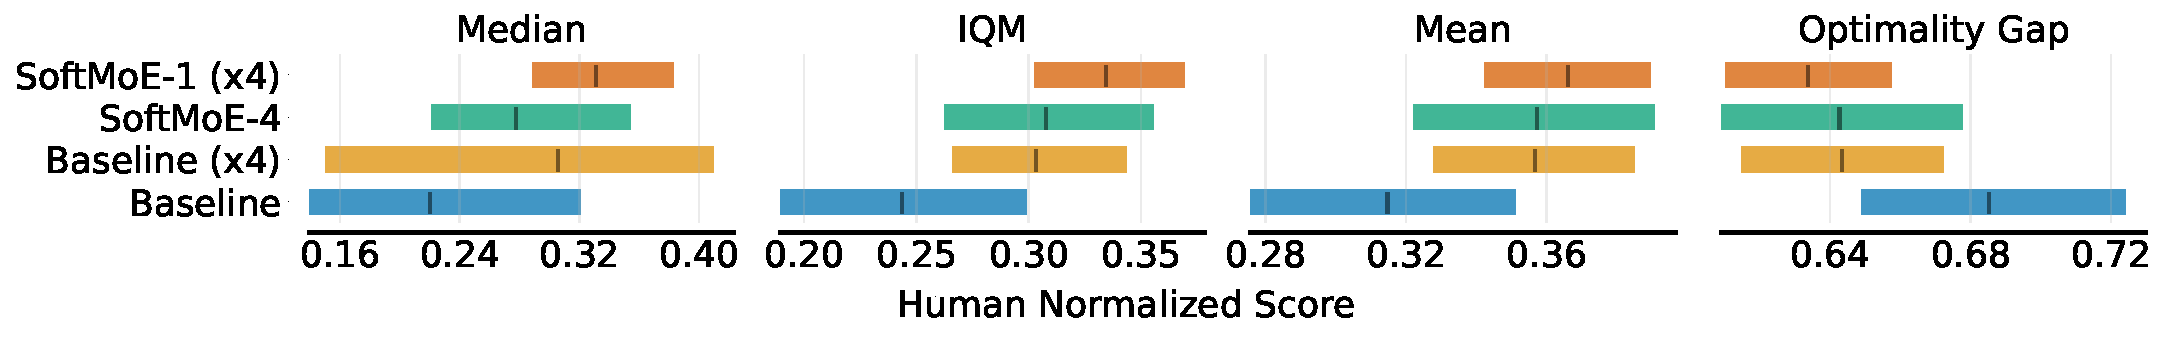
\includegraphics[width=\textwidth]{figures/results/procgenIntervalEstimates.pdf}
    \caption{\rebuttal{\textbf{Evaluating Rainbow on the 16 easy Procgen \citep{cobbe2019procgen} environments} for SoftMoE-4 and SoftMoE-1 with the penultimate layer scaled by 4x. Normalization was done using the $R_{min}$ and $R_{max}$ scores from \citet{cobbe2019procgen}. Reporting Median, IQM, Mean, and Optimality Gap \citep{agarwal2021deep}, where higher is better for the first three.   Consistent with the results in the paper, SoftMoe yields improvements, and the scaled SoftMoE-1 is comparable to SoftMoE-4.}}
    \label{fig:procgenIntEstimates}
\end{figure}

\begin{figure}[h!]
    \centering
    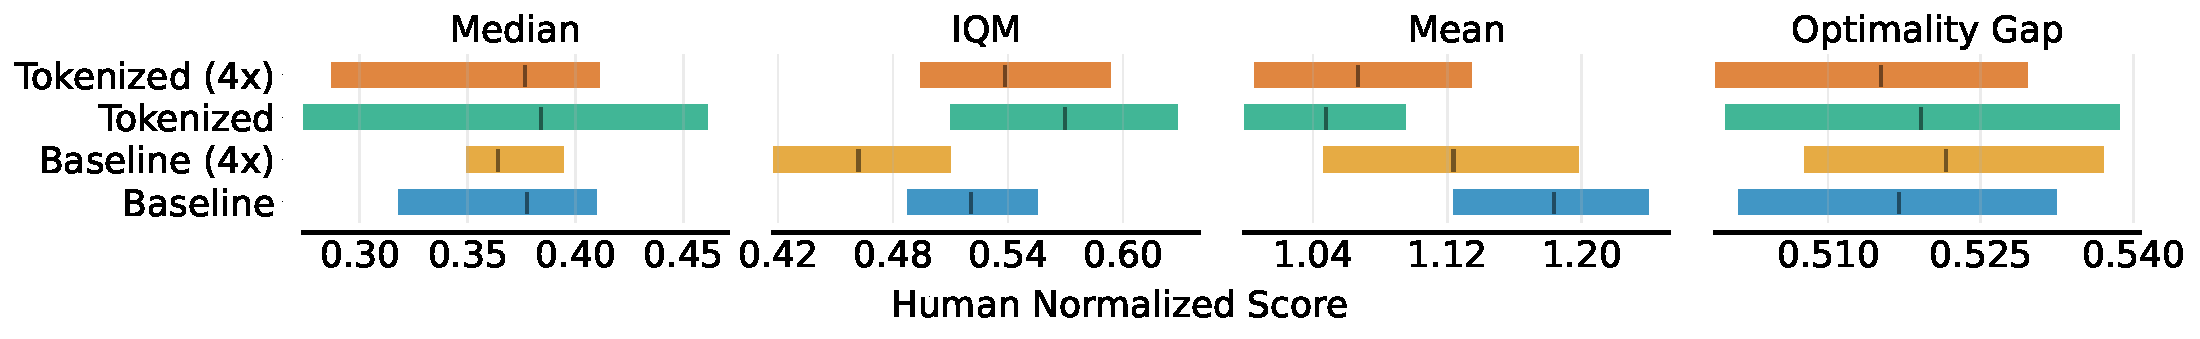
\includegraphics[width=\textwidth]{figures/results/SACCALEIntervalEstimates.pdf}
    \caption{\rebuttal{\textbf{Evaluating tokenization on the SAC encoder \citep{haarnoja2018soft} on the CALE \citep{farebrother2024cale}}, as done in Figure~\ref{fig:nonmoeexper}. In these experiments, we summed over the first dimension after tokenization. Reporting Median, IQM, Mean, and Optimality Gap \citep{agarwal2021deep}, where higher is better for the first three.    Consistent with the results in the paper, tokenization yields improvements over the baseline.}}
    \label{fig:SACCALE}
\end{figure}

\newpage
\subsection{\rebuttal{Per-game results}}
\label{sec:perGameResults}
\subsubsection{\rebuttal{Don't flatten, tokenize!}}
\begin{figure}[h!]
    \centering
    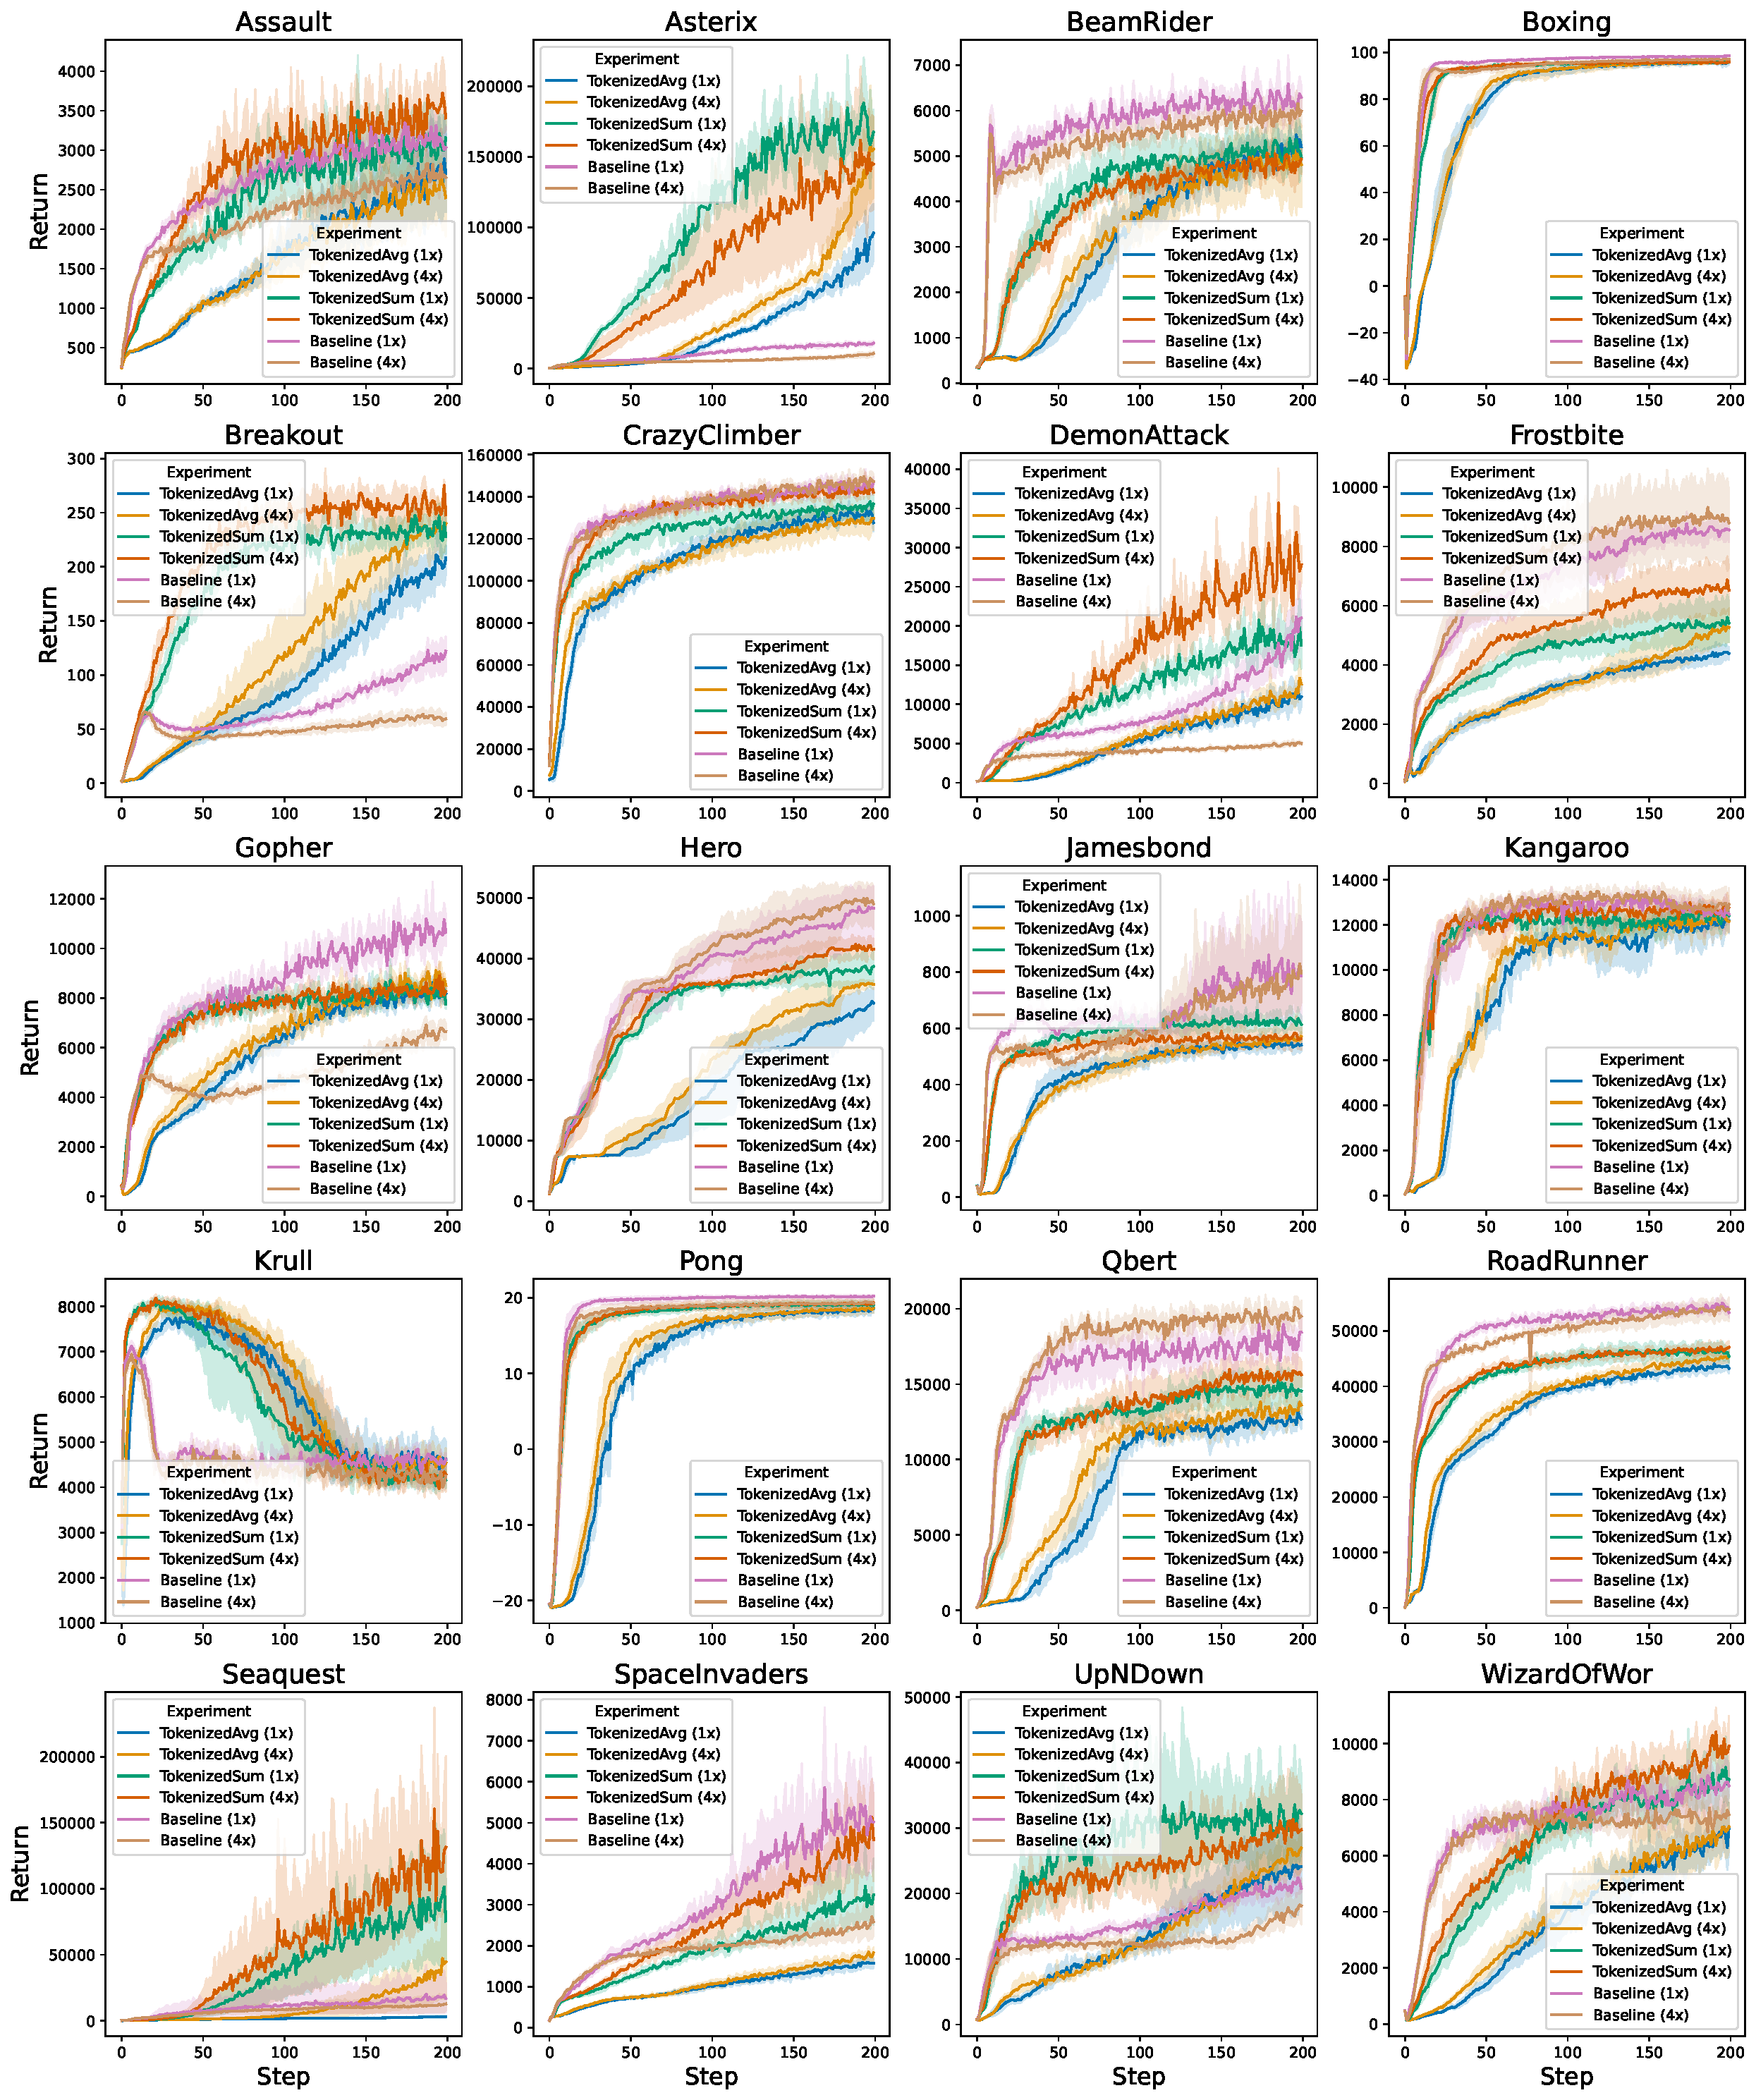
\includegraphics[width=\textwidth]{figures/results/TokenizedRainbowAllGames.pdf}
    \caption{\rebuttal{Per-game results for tokenized Rainbow-lite with CNN network (corresponding to \autoref{fig:nonmoeexper}).}}
    \label{fig:rtokenizedRainbowAllGames}
\end{figure}

\begin{figure}[h!]
    \centering
    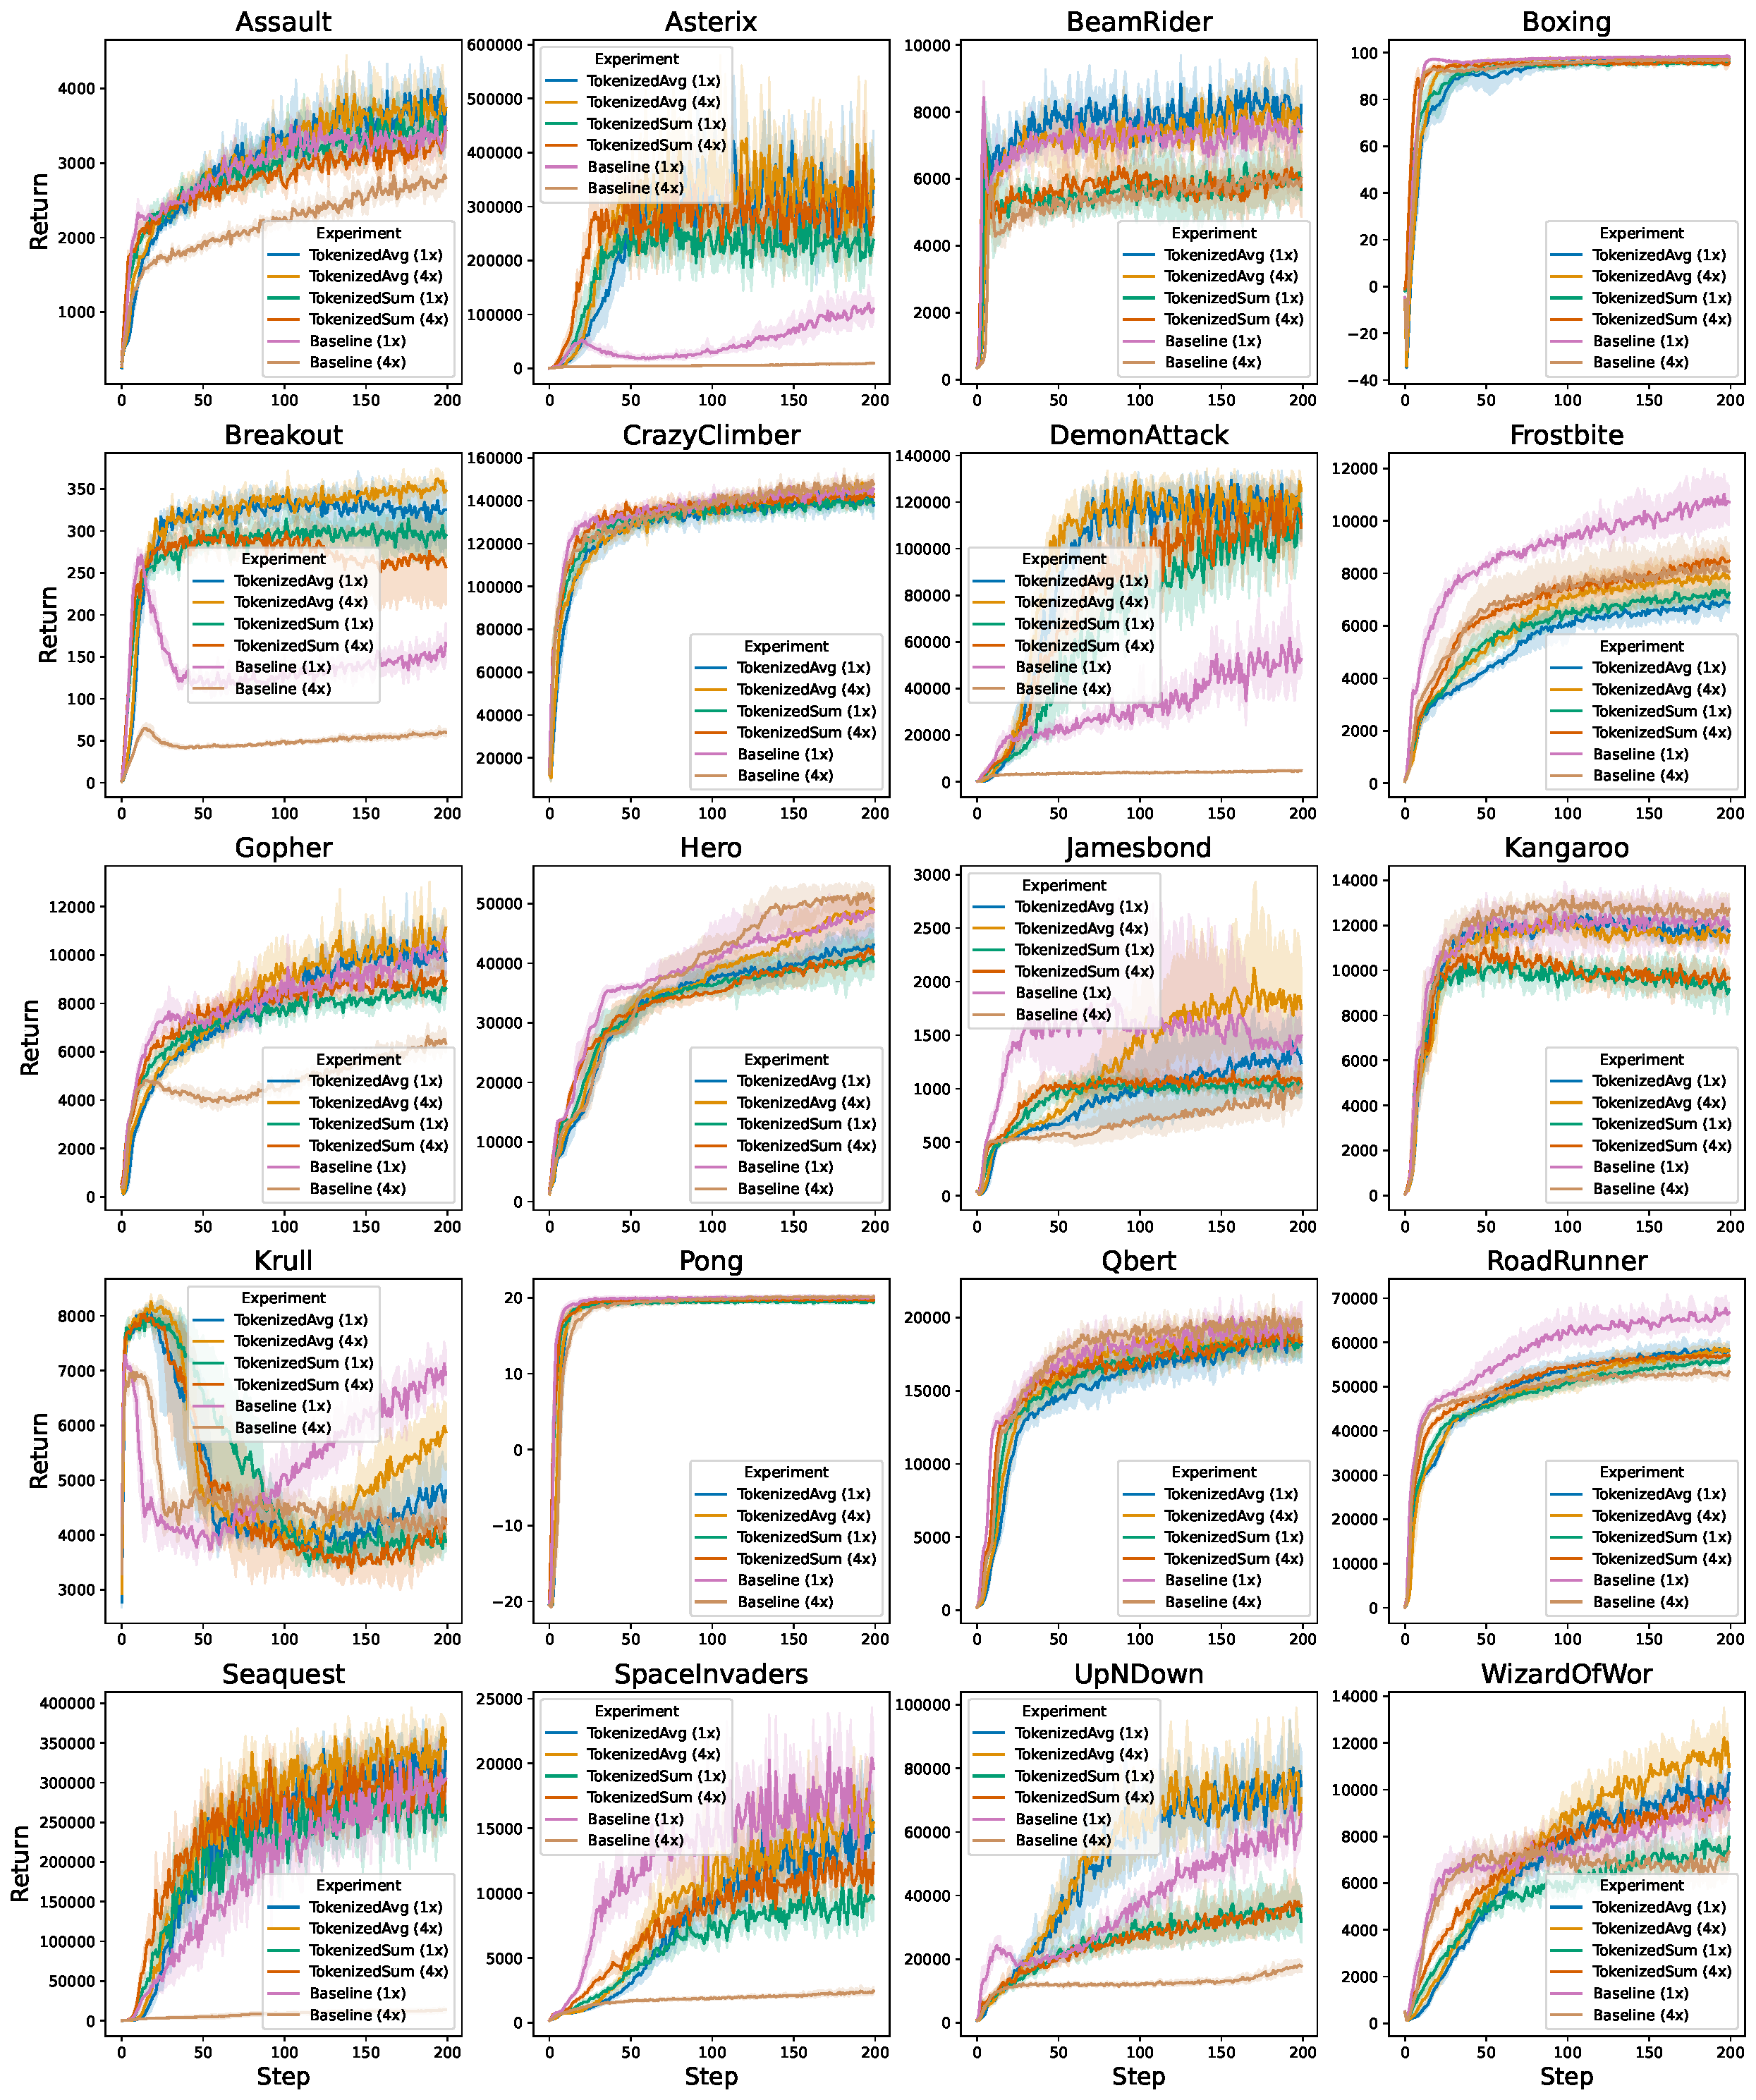
\includegraphics[width=\textwidth]{figures/results/TokenizedRainbowImpalaAllGames.pdf}
    \caption{\rebuttal{Per-game results for tokenized Rainbow-lite with Impala network (corresponding to \autoref{fig:nonmoeexper}).}}
    \label{fig:rtokenizedRainbowImpalaAllGames}
\end{figure}



% \subsection{Processing {\em combined} tokens}
% \begin{figure}[h!]
%     \centering
%     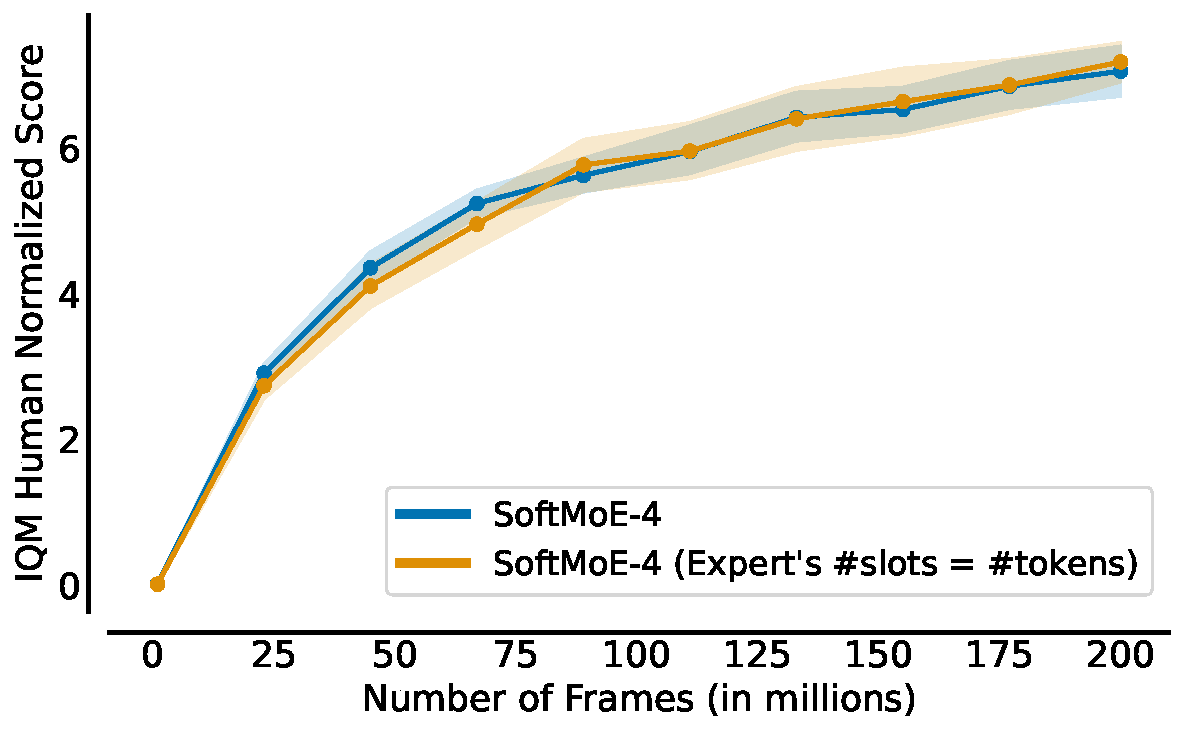
\includegraphics[width=0.45\textwidth]{figures/results/SoftMoE-4-AllTokensAllExperts.pdf}
%     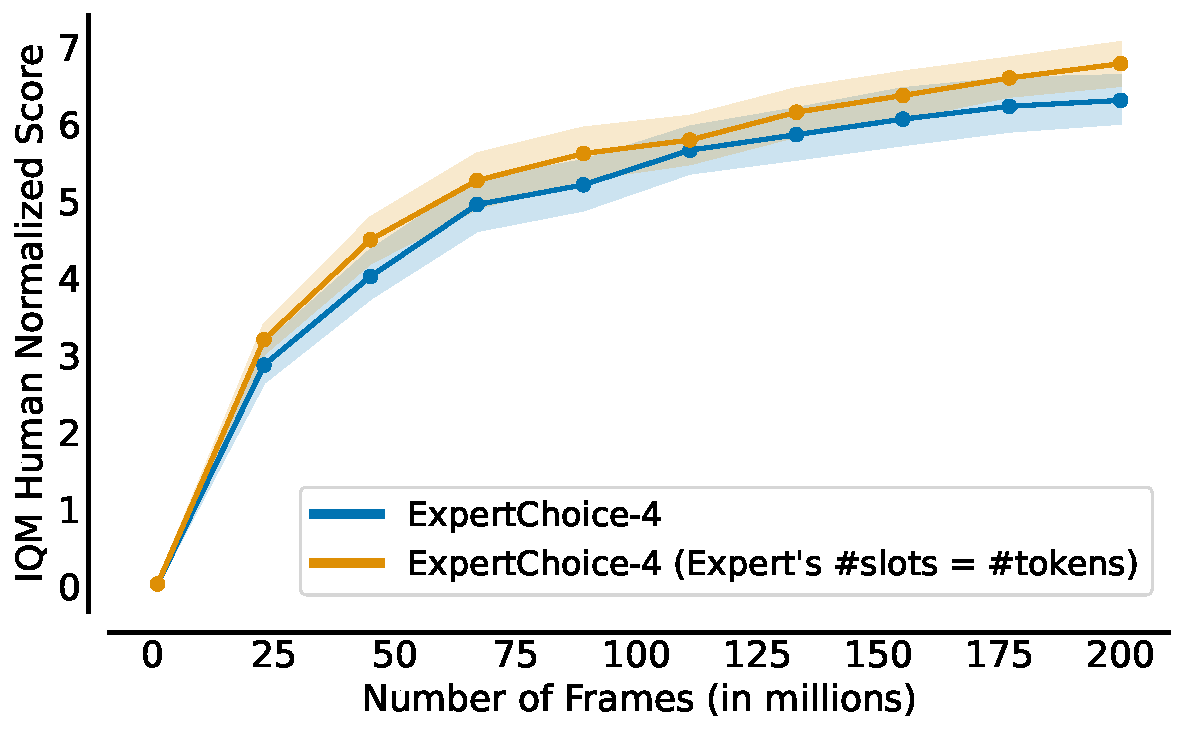
\includegraphics[width=0.45\textwidth]{figures/results/ExpertChoice_AllTokensAllExperts.pdf}
%     %\vspace{-0.4cm}
%     \caption{\textbf{Impact of expert specialization}. Even when all experts have sufficient capacity to process all tokens,  we observe no significant change in performance. This indicates that the efficiency gains of SoftMoE are not attributed to experts specializing in processing a subset of tokens.}
%     \label{fig:alltokensallexperts}
%     %\vspace{-0.2cm}
% \end{figure}
% \subsection{Expert specialization}
% \begin{figure}[h!]
%     \centering
%     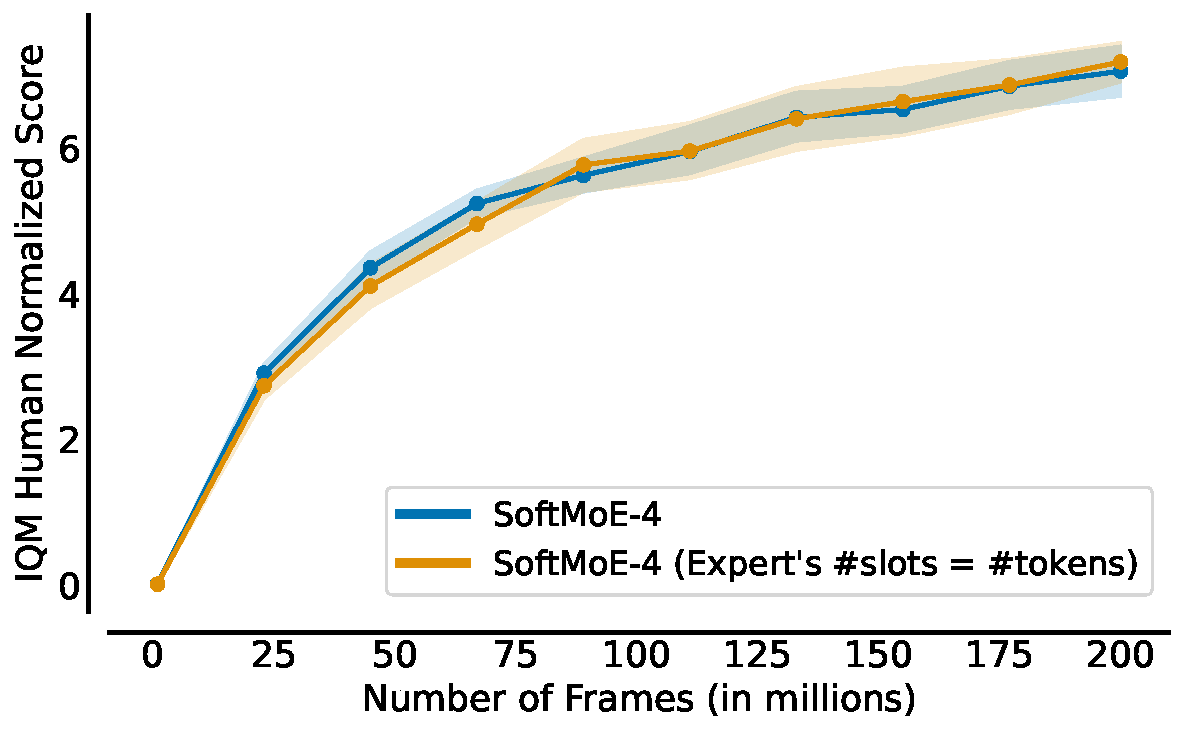
\includegraphics[width=0.45\textwidth]{figures/results/SoftMoE-4-AllTokensAllExperts.pdf}
%     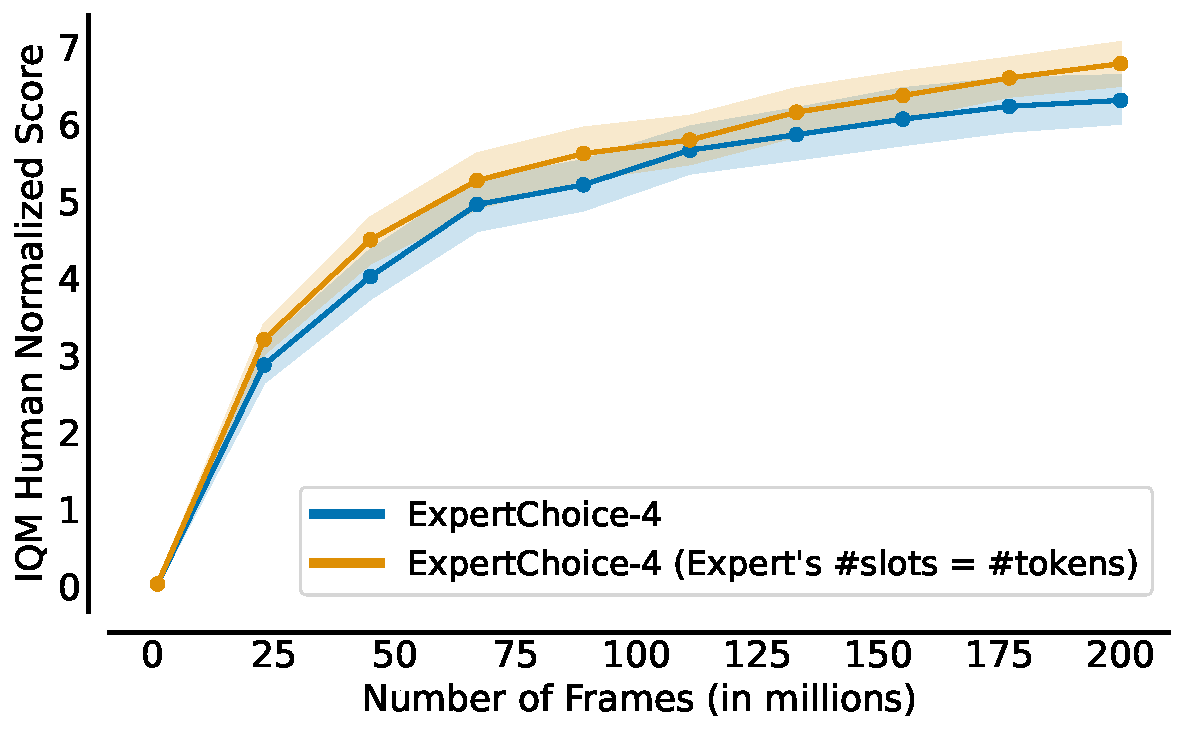
\includegraphics[width=0.45\textwidth]{figures/results/ExpertChoice_AllTokensAllExperts.pdf}
%     %\vspace{-0.4cm}
%     \caption{Impact of expert specialization. Even when all experts have sufficient capacity to process all tokens,  we observe no significant change in performance. This indicates that the efficiency gains of SoftMoE are not attributed to experts specializing in processing a subset of tokens.}
%     \label{fig:alltokensallexperts}
%     %\vspace{-0.2cm}
% \end{figure}

% \subsection{Expert width}
% \begin{figure}[h!]
%     \centering
%     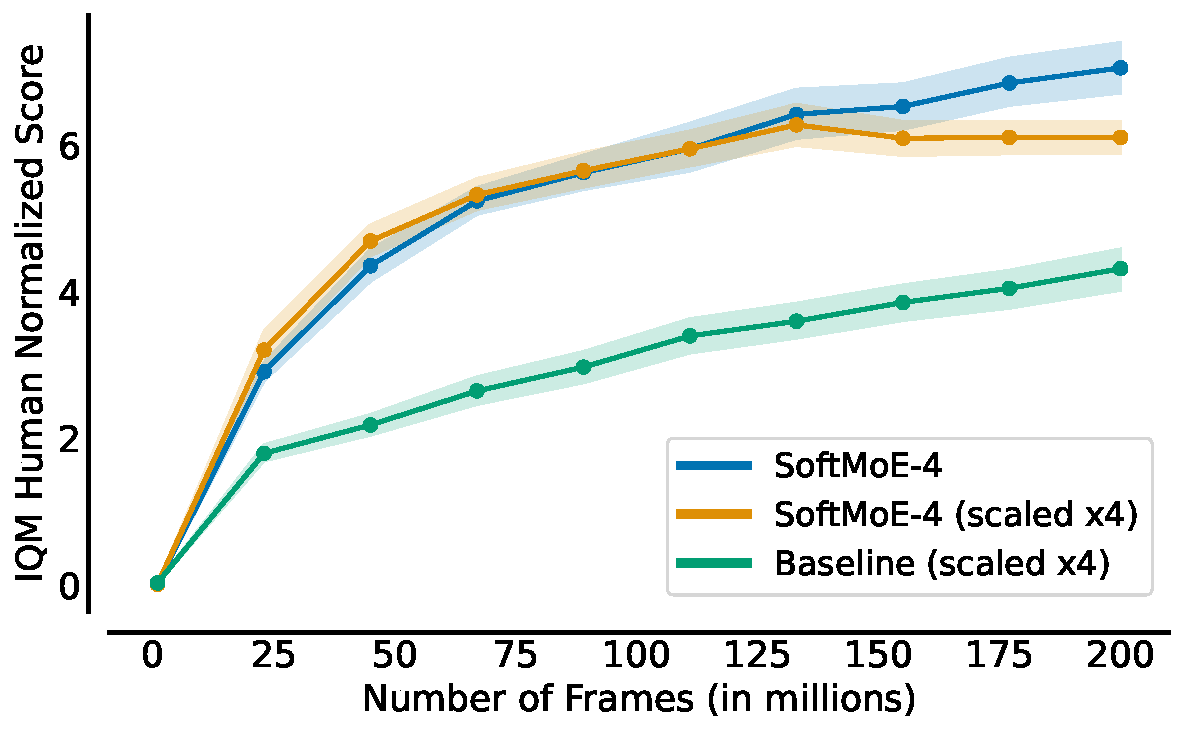
\includegraphics[width=0.65\textwidth]{figures/results/SoftMoE-4_x4.pdf}
%     %\vspace{-0.4cm}
%     \caption{\textbf{Impact of architectural dimensions}. Scaling up the expert layer dimensionality to match the \textit{width} of the scaled baseline.  Scaled experts do not suffer from the performance drop exhibited in the scaled baseline. }
%     \label{fig:expertWidth}
%     %\vspace{-0.2cm}
% \end{figure}

% \subsection{Network depth}
% \begin{figure}[h!]
%     \centering
%     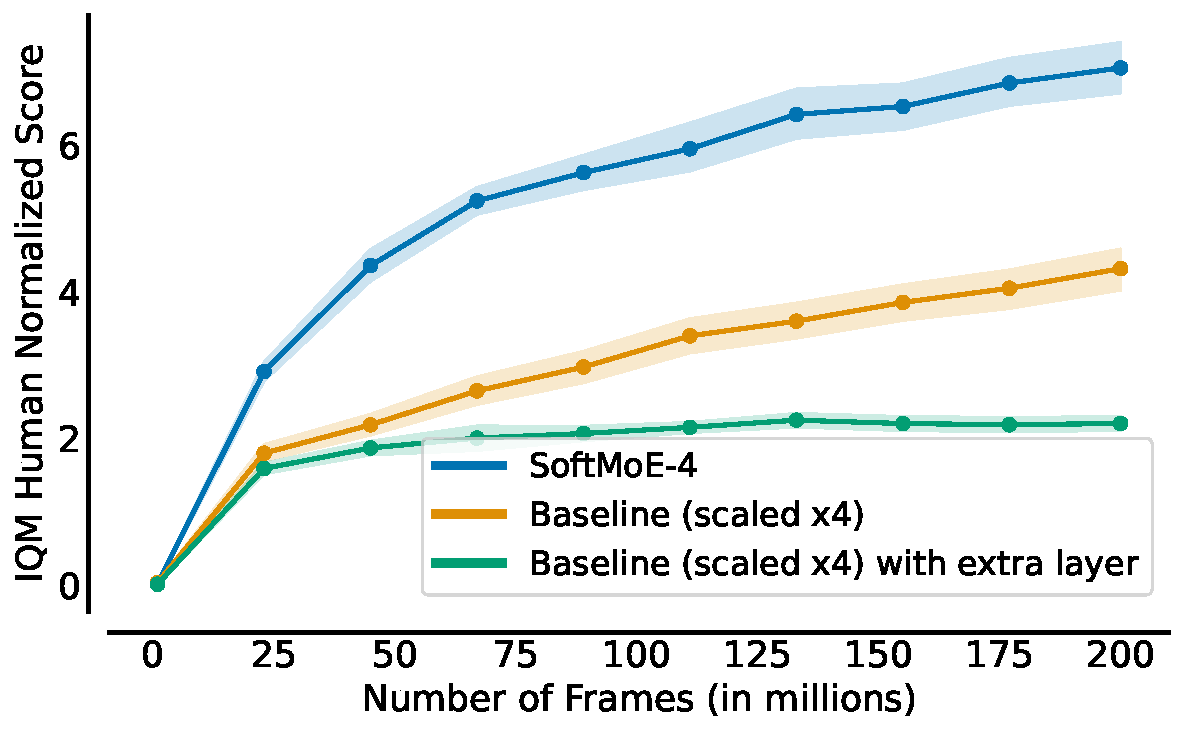
\includegraphics[width=0.65\textwidth]{figures/results/SoftMoE-x4_vs_Baseline_w_extralayer.pdf}
%     %\vspace{-0.4cm}
%     \caption{\textbf{Impact of architectural dimensions}. Adding an extra layer to the baseline to match the SoftMoE network \textit{depth} does not lead to the performance improvements achieved by the latter. \todo{left still running}}
%     \label{fig:networkDepth}
%     %\vspace{-0.2cm}
% \end{figure}



% \section{Don't flatten, tokenize! Extra results}
% \subsection{Combined tokenization is a key driver}


% \begin{figure}[h!]
%     \centering
%         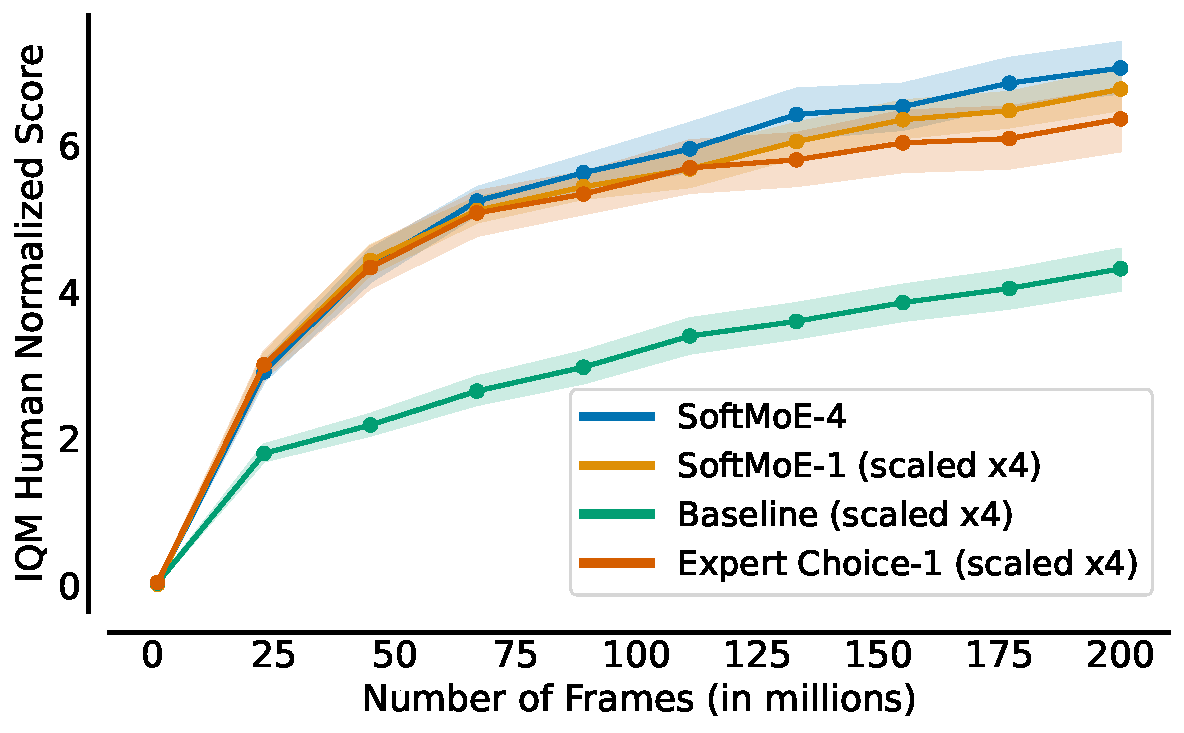
\includegraphics[width=0.45\textwidth]{figures/results/SoftMoE-1_x4.pdf} 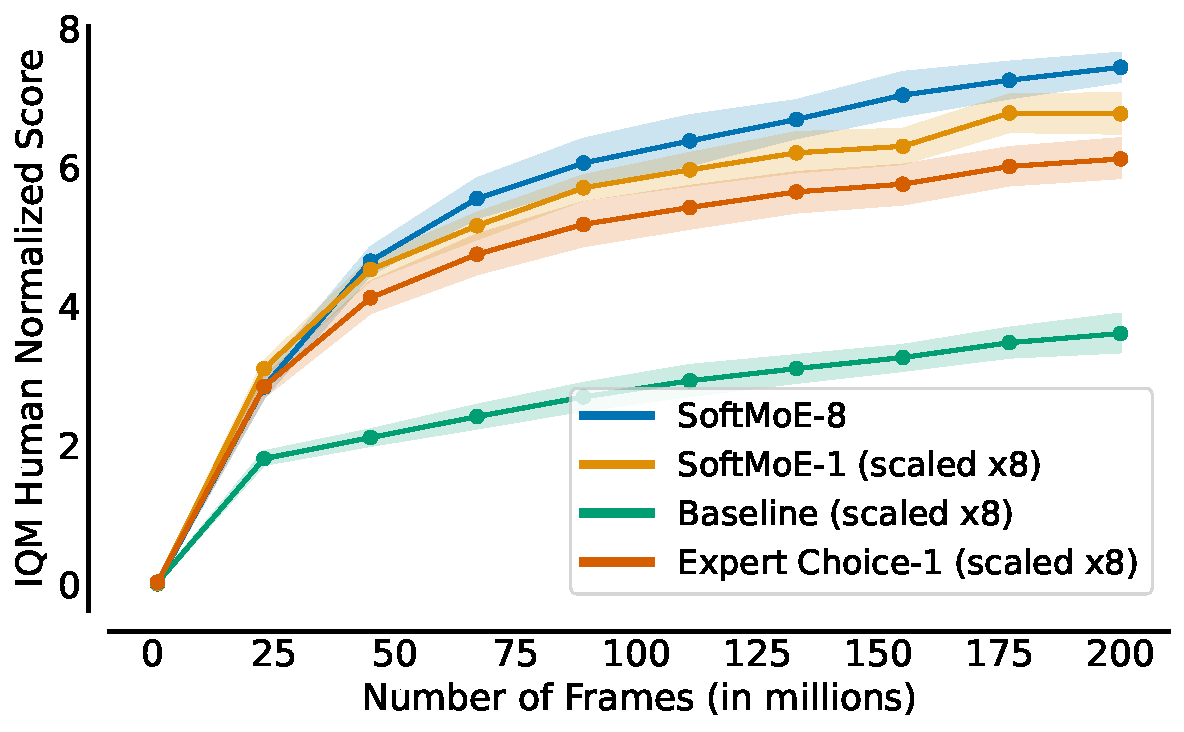
\includegraphics[width=0.45\textwidth]{figures/results/SoftMoE-1_x8.pdf}
%     %\vspace{-0.4cm}
%     \caption{\textbf{Combined tokenization is a key driver of SoftMoE's efficacy.} 4x (left) and 8x (right) scaled SoftMoE-1 can approximate the performance of multiple experts. Even \textit{Non-combined} tokenization with single expert (Expert Choice-1) surpasses the baseline considerably, highlighting the crucial role of tokenization.}
%     \label{fig:1expertvsmultipleexperts8}
%     %\vspace{-0.2cm}
% \end{figure}


% \begin{figure}[h!]
%     \centering
%     % 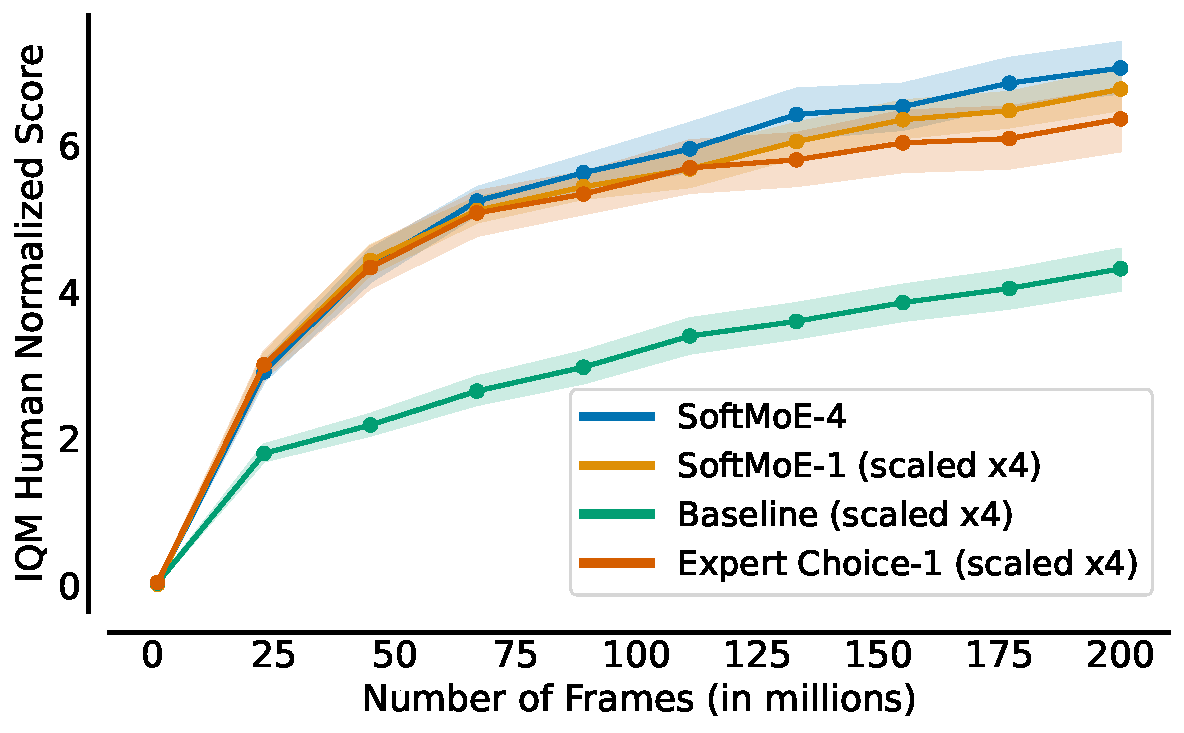
\includegraphics[width=0.45\textwidth]{figures/results/SoftMoE-1_x4.pdf}
%     %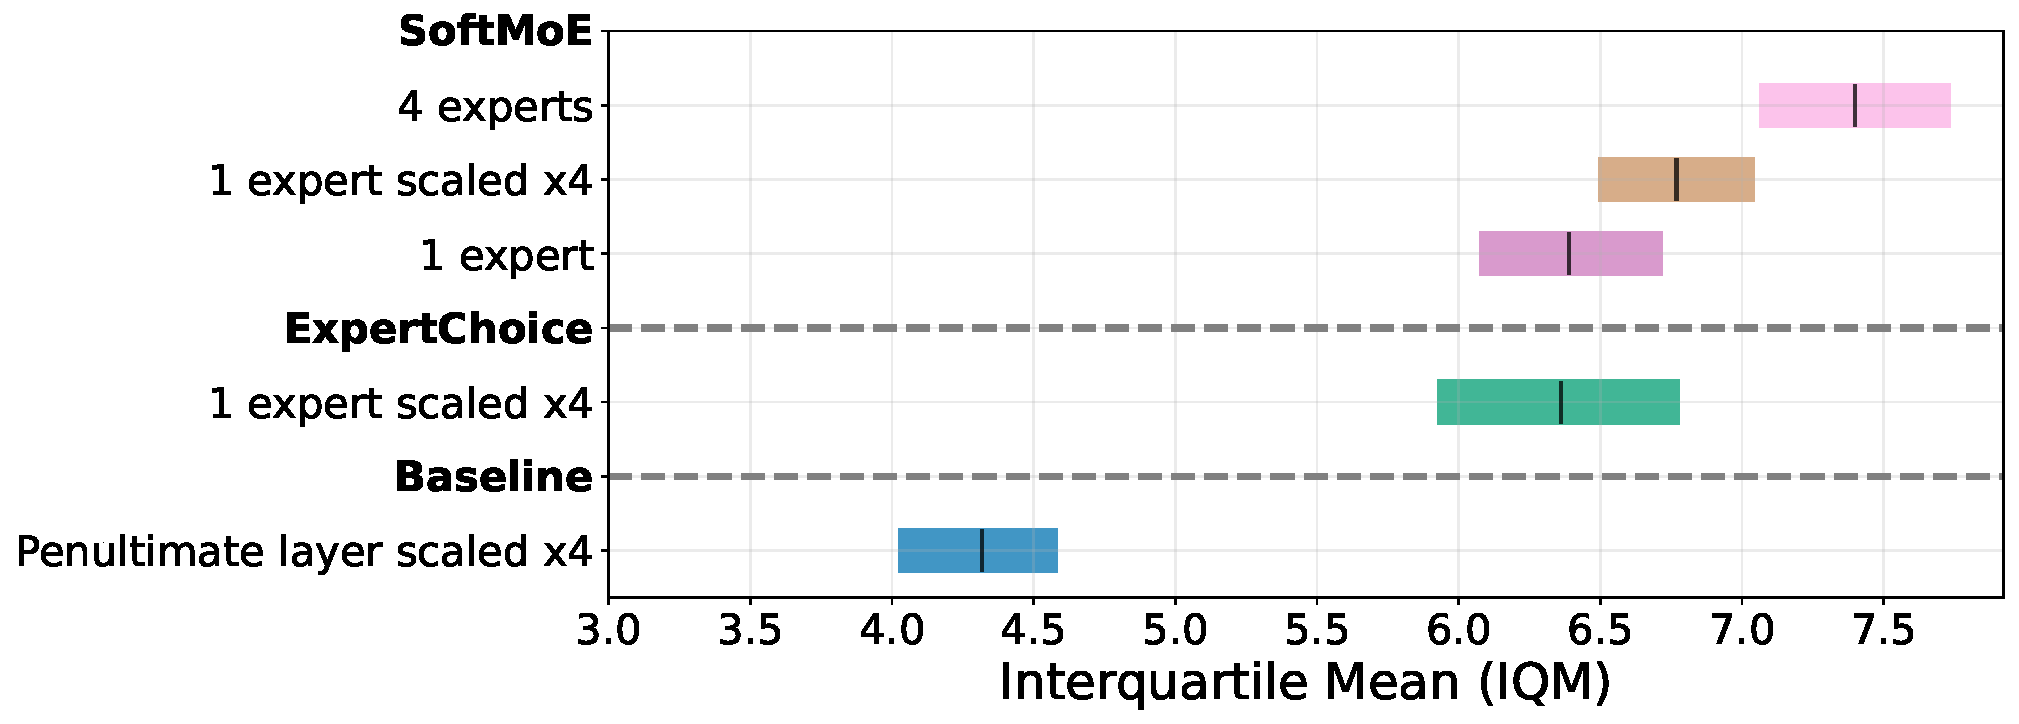
\includegraphics[width=0.55\textwidth]{figures/results/section5_aggregate_v2_4experts.pdf}
%     % 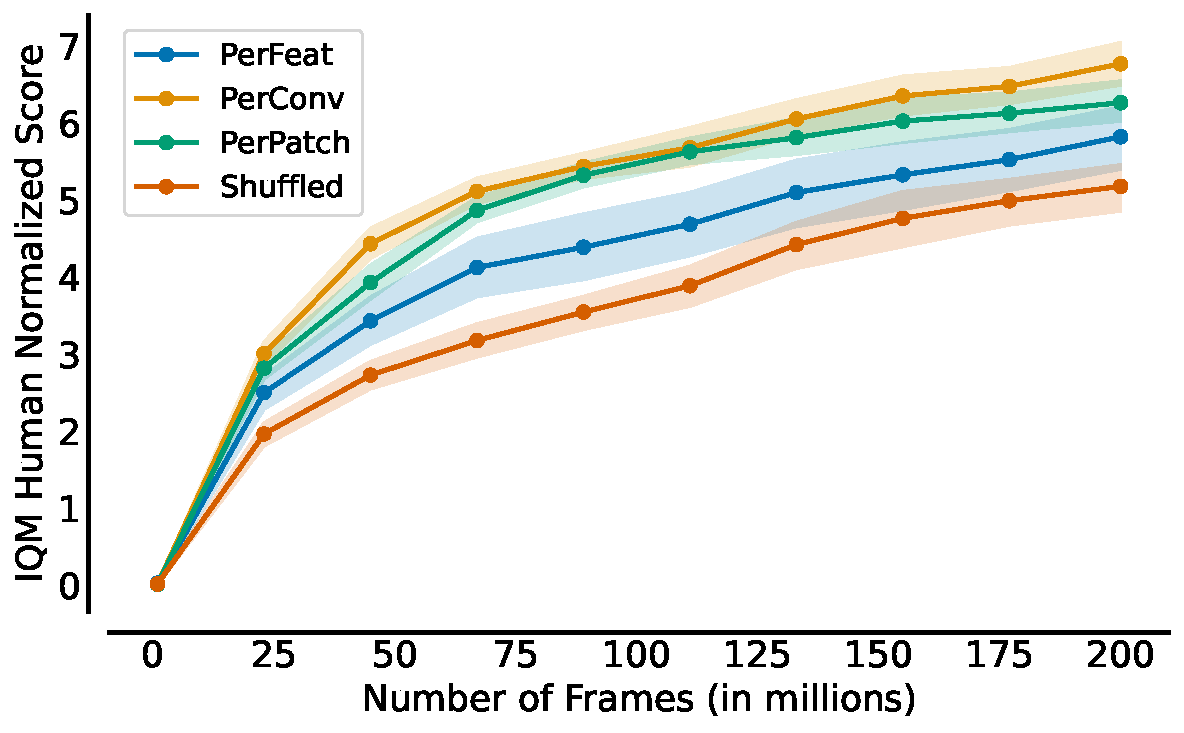
\includegraphics[width=0.45\textwidth]{figures/results/token_types_1expertx4.pdf}
%     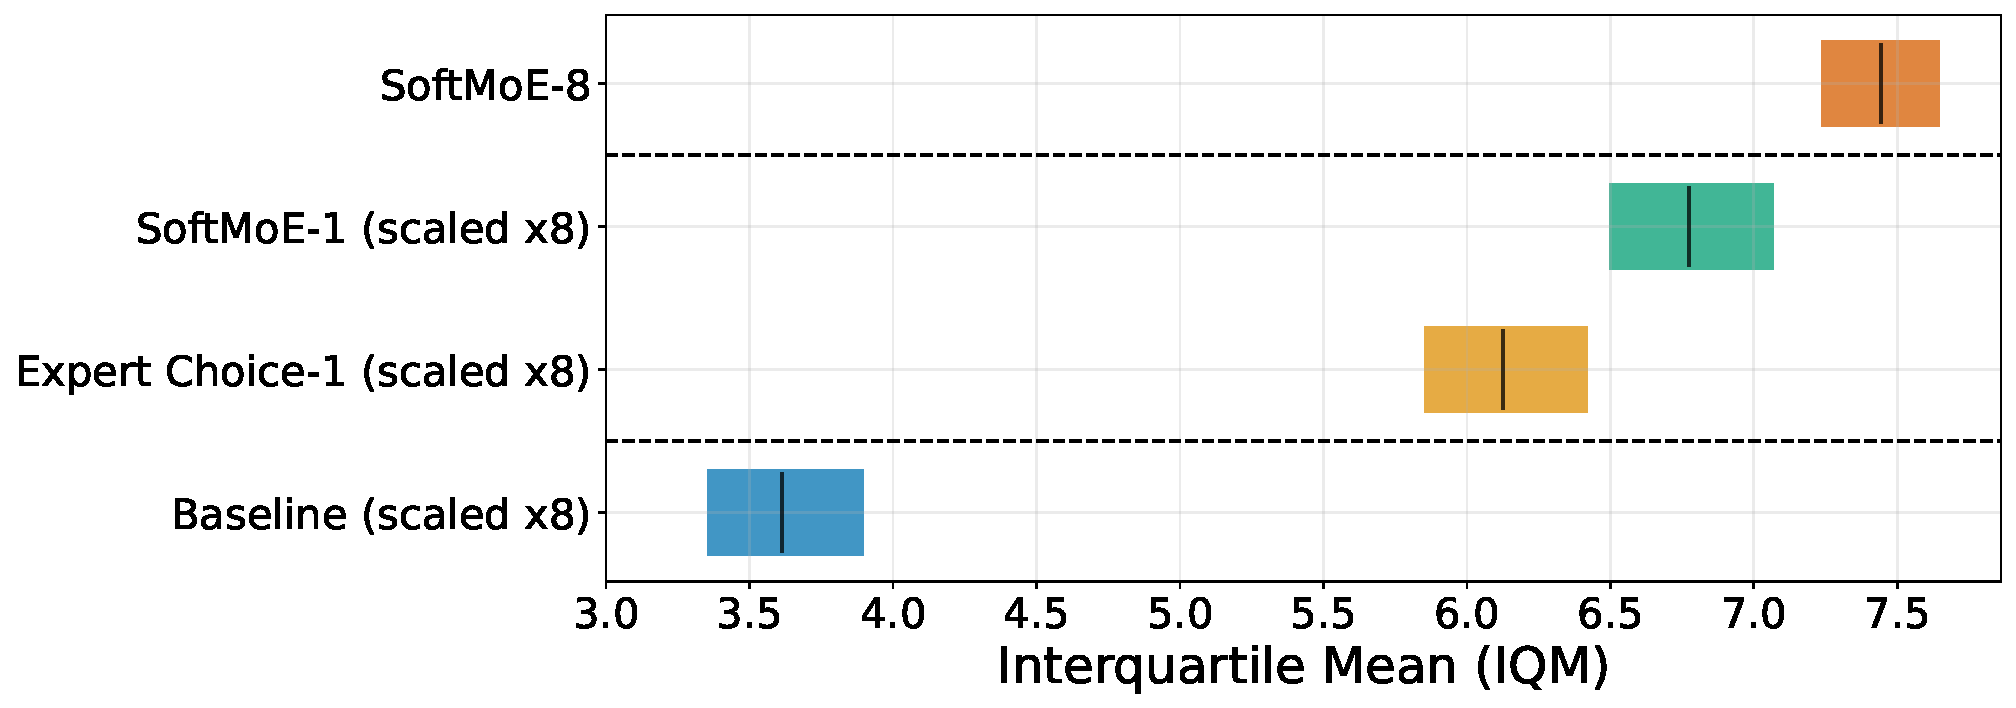
\includegraphics[width=0.44\textwidth]{figures/results/section5_aggregate_v2_8experts.pdf}
%     %\vspace{-0.4cm}
%     \caption{\textbf{Combined tokenization is a key driver of SoftMoE's efficacy}. Scaled SoftMoE-1 can approximate the performance of multiple experts. Even \textit{Non-combined} tokenization with single expert (Expert Choice-1) surpasses the baseline considerably, highlighting the crucial role of tokenization. \todo{update figure}}
%     \label{fig:1expertvsmultipleexperts_x8}
%     %\vspace{-0.2cm}
% \end{figure}

% \subsection{Additional analyses - extra results}
% \subsection{Are all types of tokenization equally effective?}

% \begin{figure}[h!]
%     \centering
%     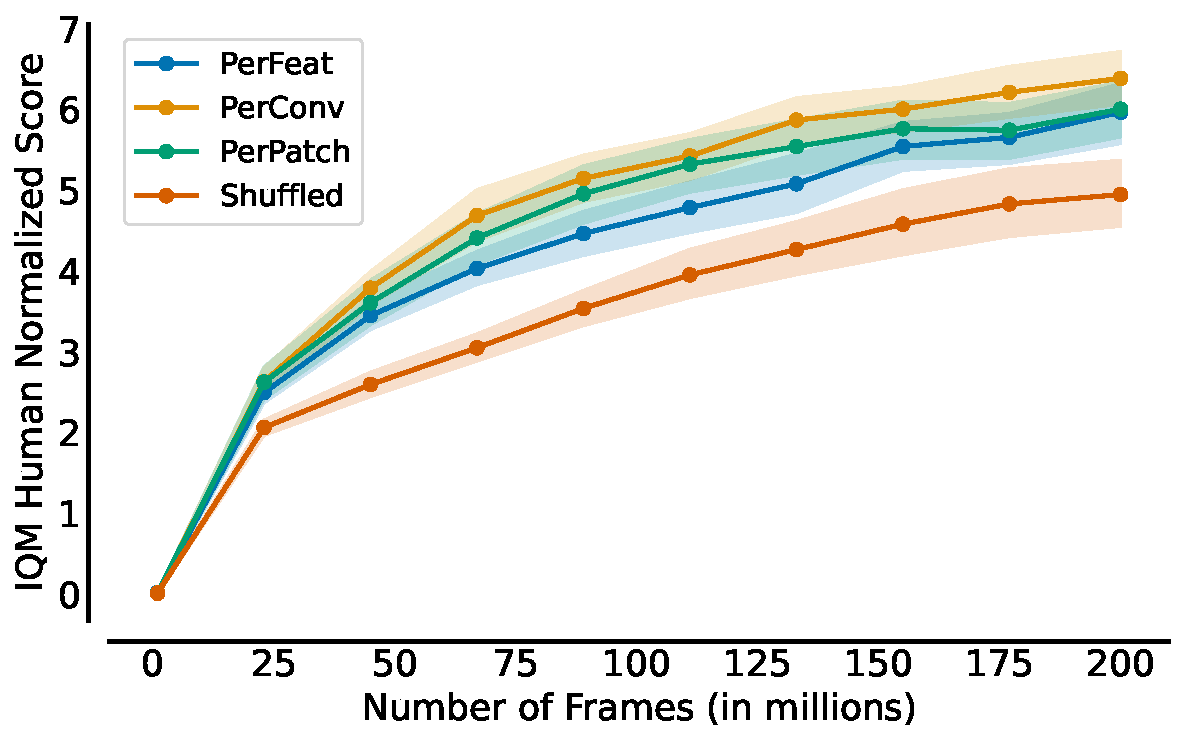
\includegraphics[width=0.45\textwidth]{figures/results/token_types_1expert.pdf}
%     %\vspace{-0.4cm}
%     \caption{\textbf{Comparison of different token types for SoftMoE-1} with penultimate layer of the standard size. PerConv achieves the highest performance, suggesting that maintaining the spatial structure of the features plays a role on the observed benefits.}
%     \label{fig:tokentypes}
%     %\vspace{-0.2cm}
% \end{figure}


% \paragraph{\textcolor{red}{Optional - maybe appendix}Not all features/tokens are important}
% maybe here we add the baseline and sparsity 

% \begin{figure}[h!]
%     \centering
%     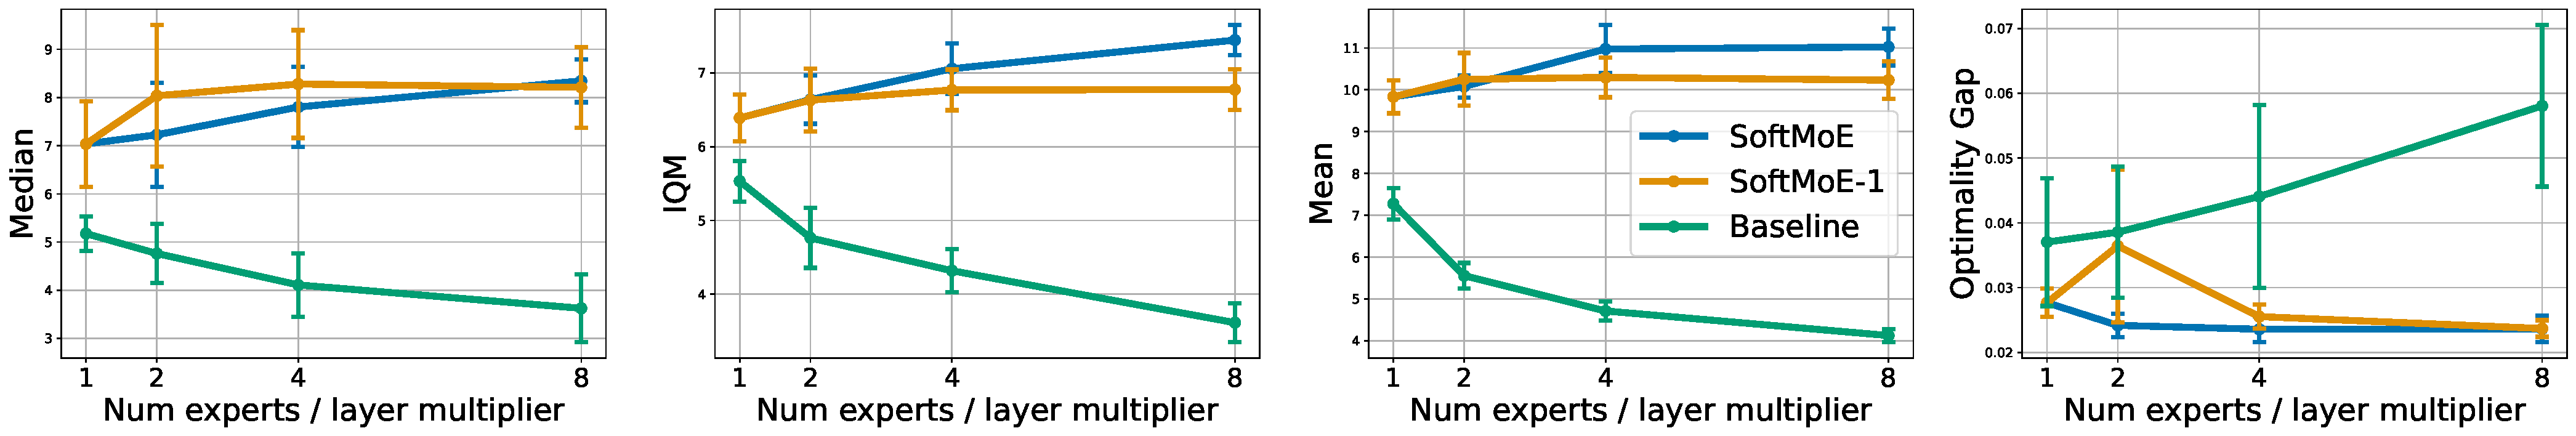
\includegraphics[width=\textwidth]{figures/results/aggregate_comparison.pdf}
%     %\vspace{-0.4cm}
%     \caption{\textcolor{red}{maybe just one of the four}}
%     \label{fig:mainfig_all_metrics}
%     %\vspace{-0.2cm}
% \end{figure}

% \begin{figure}
%     \centering
%     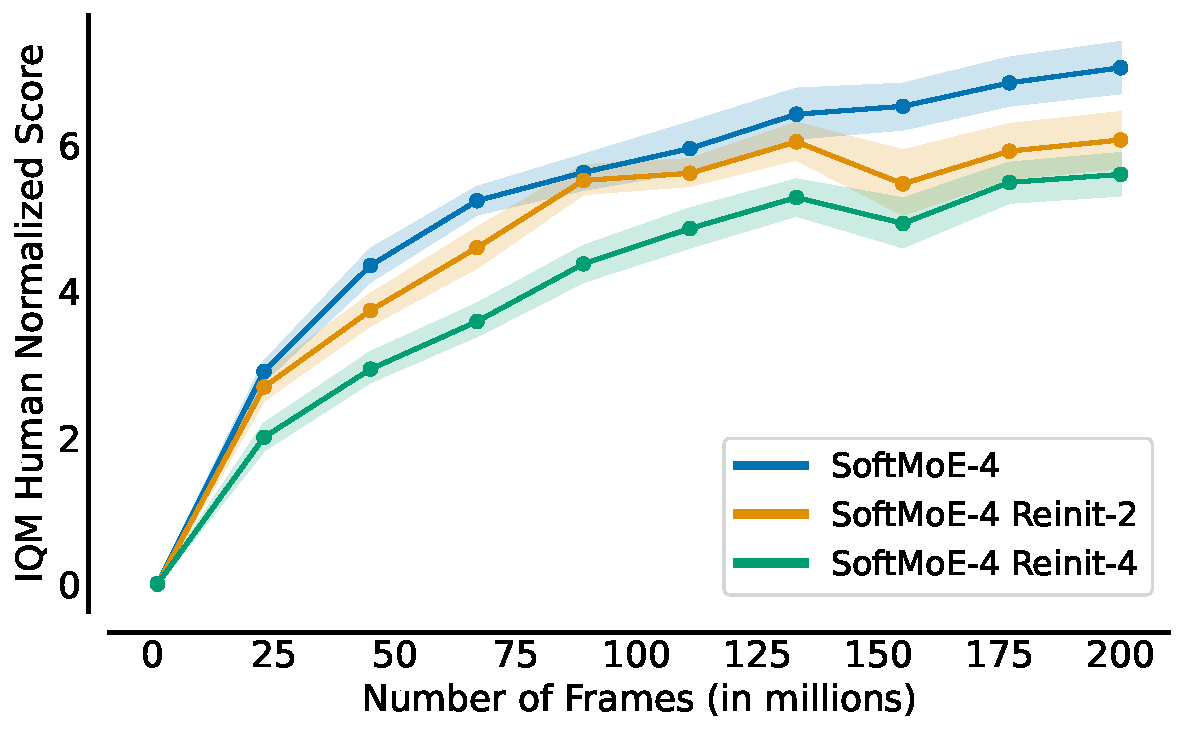
\includegraphics[width=0.45\textwidth]{figures/results/SoftMoE-4_Rainbow-Reset-all.pdf}

%     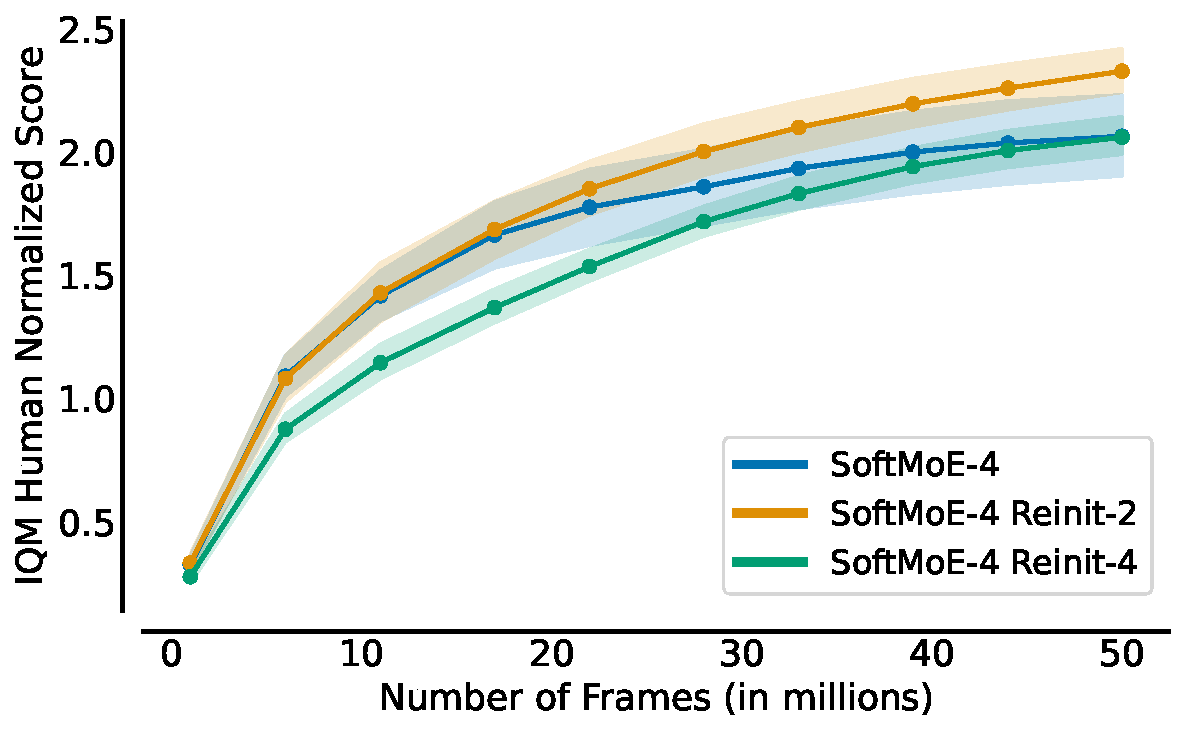
\includegraphics[width=0.45\textwidth]{figures/results/SoftMoE-4_DER-Reset-all.pdf}

%     %\vspace{-0.4cm}
%     \caption{\todo{reset (left) rainbow (right)DER ,  (left)  }}
%     \label{fig:reset_DER}
%     %\vspace{-0.2cm}
% \end{figure}
